\documentclass[a4paper,11pt]{article}
\usepackage{listings}
\usepackage[utf8]{inputenc}
\usepackage[spanish]{babel}

\decimalpoint
\usepackage{dcolumn}
\newcolumntype{.}{D{.}{\esperiod}{-1}}
\makeatletter
\addto\shorthandsspanish{\let\esperiod\es@period@code}
\makeatother

\RequirePackage{verbatim}
\usepackage{fancyhdr}
\usepackage{graphicx}
\usepackage{afterpage}
\usepackage{dirtytalk}
\usepackage{longtable}
\usepackage[font=scriptsize,labelfont=bf]{caption}
\usepackage[
backend=biber,
sorting=ynt
]{biblatex}
\addbibresource{bibliografia.bib}

\usepackage[hidelinks]{hyperref}
\usepackage[dvipsnames]{xcolor}
\usepackage{csquotes}
\usepackage{pdflscape}
\usepackage{listings}
\usepackage{subcaption}
\usepackage{wrapfig}

% ********************************************************************
% Re-usable information
% ********************************************************************
\newcommand{\myTitle}{Aplicación Distribuida Basada en Blockchain para dar soporte a IoT\xspace}
\newcommand{\mySubTitle}{Desarrollo de un registro distribuido para IoT usando la tecnología Blockchain\xspace}
\newcommand{\myDegree}{Grado en Ingeniería Informática\xspace}
\newcommand{\myName}{Fernando Rafael Talavera Mendoza)\xspace}
\newcommand{\myProf}{Pedro Ángel Castillo Valdivieso\xspace}
\newcommand{\myFaculty}{Escuela Técnica Superior de Ingenierías Informática y de
Telecomunicación\xspace}
\newcommand{\myFacultyShort}{E.T.S. de Ingenierías Informática y de
Telecomunicación\xspace}
\newcommand{\myDepartment}{Departamento de Arquitectura y Tecnología de Computadores\xspace}
\newcommand{\myUni}{\protect{Universidad de Granada}\xspace}
\newcommand{\myLocation}{Granada\xspace}
\newcommand{\myTime}{\today\xspace}
\newcommand{\myVersion}{Version 0.1\xspace}
\usepackage{url}
\usepackage{colortbl,longtable}
\usepackage[stable]{footmisc}

\pagestyle{fancy}
\fancyhf{}
\fancyhead[LO]{\nouppercase{\leftmark}}
\fancyfoot[LE,RO]{\thepage}

\setlength{\headheight}{1.5\headheight}

\newcommand{\HRule}{\rule{\linewidth}{0.5mm}}

\definecolor{gray97}{gray}{.97}
\definecolor{gray75}{gray}{.75}
\definecolor{gray45}{gray}{.45}
\definecolor{gray30}{gray}{.94}

\lstset{ frame=Ltb,
     framerule=0.5pt,
     aboveskip=0.5cm,
     framextopmargin=3pt,
     framexbottommargin=3pt,
     framexleftmargin=0.1cm,
     framesep=0pt,
     rulesep=.4pt,
     backgroundcolor=\color{gray97},
     rulesepcolor=\color{black},
     %
     stringstyle=\ttfamily,
     showstringspaces = false,
     basicstyle=\scriptsize\ttfamily,
     commentstyle=\color{gray45},
     keywordstyle=\bfseries,
     %
     numbers=left,
     numbersep=6pt,
     numberstyle=\tiny,
     numberfirstline = false,
     breaklines=true,
   }
 
% minimizar fragmentado de listados
\lstnewenvironment{listing}[1][]
   {\lstset{#1}\pagebreak[0]}{\pagebreak[0]}

\lstdefinestyle{CodigoC}
   {
	basicstyle=\scriptsize,
	frame=single,
	language=C,
	numbers=left
   }
\lstdefinestyle{CodigoC++}
   {
	basicstyle=\small,
	frame=single,
	backgroundcolor=\color{gray30},
	language=C++,
	numbers=left
   }

 
\lstdefinestyle{Consola}
   {basicstyle=\scriptsize\bf\ttfamily,
    backgroundcolor=\color{gray30},
    frame=single,
    numbers=none
   }


\newcommand{\bigrule}{\titlerule[0.5mm]}

%Para conseguir que en las páginas en blanco no ponga cabeceras
\makeatletter
\def\clearpage{%
  \ifvmode
    \ifnum \@dbltopnum =\m@ne
      \ifdim \pagetotal <\topskip
        \hbox{}
      \fi
    \fi
  \fi
  \newpage
  \thispagestyle{empty}
  \write\m@ne{}
  \vbox{}
  \penalty -\@Mi
}
\makeatother

\newcommand\myemptypage{
    \null
    \thispagestyle{empty}
    \addtocounter{page}{-1}
    \newpage
}

\usepackage{pdfpages}
\begin{document}
\begin{titlepage}
 
\newlength{\centeroffset}
\setlength{\centeroffset}{-0.5\oddsidemargin}
\addtolength{\centeroffset}{0.5\evensidemargin}

\noindent\hspace*{\centeroffset}\begin{minipage}{\textwidth}

\centering

\includegraphics[width=0.9\textwidth]{imagenes/logo_ugr}\\[1.4cm]

\textsc{ \Large TRABAJO FIN DE GRADO\\[0.2cm]}
\textsc{ INGENIERÍA EN INGENIERÍA INFORMÁTICA}\\[1cm]
% Upper part of the page
% 
% Title
{\LARGE\bfseries Aplicación Distribuida Basada en Blockchain para dar soporte a IoT\\
}
\noindent\rule[-1ex]{\textwidth}{3pt}\\[3.5ex]
{\large\bfseries Desarrollo de un registro distribuido para IoT usando la tecnología Blockchain.}
\end{minipage}

\vspace{2.5cm}
\noindent\hspace*{\centeroffset}\begin{minipage}{\textwidth}
\centering

\textbf{Autor}\\ {Fernando Rafael Talavera Mendoza}\\[2.5ex]
\textbf{Director}\\
{Pedro Ángel Castillo Valdivieso}\\[2cm]

\includegraphics[width=0.3\textwidth]{imagenes/etsiit_logo}\\[0.1cm]
\textsc{Escuela Técnica Superior de Ingenierías Informática y de Telecomunicación}\\
\textsc{---}\\
Granada, Noviembre de 2020
\end{minipage}
%\addtolength{\textwidth}{\centeroffset}
%\vspace{\stretch{2}}
\end{titlepage}



\myemptypage
\begin{titlepage}

\setlength{\centeroffset}{-0.5\oddsidemargin}
\addtolength{\centeroffset}{0.5\evensidemargin}

\noindent\hspace*{\centeroffset}\begin{minipage}{\textwidth}

\centering

%si el proyecto tiene logo poner aquí

\includegraphics[width=0.9\textwidth]{imagenes/logo_ugr}\\[1.4cm]

% Title

{\Huge\bfseries Aplicación Distribuida Basada en Blockchain para dar soporte a IoT\\
}
\noindent\rule[-1ex]{\textwidth}{3pt}\\[3.5ex]
{\large\bfseries Desarrollo de un registro distribuido para IoT usando la tecnología Blockchain.\\[4cm]}
\end{minipage}

\vspace{2.5cm}
\noindent\hspace*{\centeroffset}\begin{minipage}{\textwidth}
\centering

\textbf{Autor}\\ {Fernando Rafael Talavera Mendoza}\\[2.5ex]
\textbf{Director}\\
{Pedro Ángel Castillo Valdivieso}\\[2cm]


\includegraphics[width=0.2\textwidth]{imagenes/atc}\\[0.1cm]
\textsc{Departamento de Arquitectura y Tecnología de Computadores}\\
\textsc{---}\\
Granada, Noviembre de 2020
\end{minipage}
%\addtolength{\textwidth}{\centeroffset}
\end{titlepage}




\myemptypage
\thispagestyle{empty}

\begin{center}
{\large\bfseries Aplicación Distribuida Basada en Blockchain para dar soporte a IoT}\\
\end{center}
\begin{center}
Fernando Rafael Talavera Mendoza\\
\end{center}

%\vspace{0.7cm}
\noindent{\textbf{Palabras clave}: Blockchain, Raspberry Pi, Hyperledger Fabric, Docker, GraphQL, Gatsby.}

\vspace{0.7cm}
\noindent{\textbf{Resumen}}

\vspace{5mm}

Desde el comienzo de Bitcoin, la tecnología Blockchain surgió como la siguiente tecnología revolucionaria. 
Aunque Blockchain comenzó como una tecnología central de Bitcoin, sus casos de uso se están expandiendo a 
muchas otras áreas, incluyendo finanzas, Internet de las cosas, seguridad y demás. Cabe destacar, que la 
tecnología del Internet de las cosas ha tenido gran influencia y aceptación, y actualmente, muchos sectores 
públicos y privados se están sumergiendo en la tecnología. Estos dispositivos necesitan comunicarse y 
sincronizarse entre sí. Pero en situaciones en las que más de miles o decenas de miles de dispositivos que se 
conectan, esperamos que el uso del modelo actual de cliente-servidor pueda tener limitaciones y problemas 
durante la sincronización. 

\vspace{5mm}

\noindent Por tanto, se propone usar la tecnología Blockchain para controlar y configurar los dispositivos 
de IoT. Realizar un estudio del papel que puede tomar en dicho escenario, a nivel de soluciones, benefios 
y desafíos. Y escoger las herramientas para realizar una prueba de concepto con Raspberry Pi e implementar
una aplicación distribuida para facilitar el registro y la administración de los dispositivos a los 
usuarios en una red domótica.

\newpage
\thispagestyle{empty}

\begin{center}
{\large\bfseries Distributed Application Based on Blockchain to support IoT: Development of a distributed registry for 
IoT using Blockchain technology.}\\
\end{center}
\begin{center}
Fernando Rafael Talavera Mendoza\\
\end{center}

%\vspace{0.7cm}
\noindent{\textbf{Keywords}: Blockchain, Raspberry Pi, Hyperledger Fabric, Docker, GraphQL, Gatsby.}

\vspace{0.7cm}
\noindent{\textbf{Abstract}}

\vspace{5mm}

Since the start of Bitcoin in 2008, blockchain technology emerged as the next revolutionary technology. 
Though blockchain started off as a core technology of Bitcoin, its use cases are expanding to many other 
areas including finances, Internet of Things (IoT), security and such. It is noteworthy, that IoT technology 
has had great influence and acceptance, and currently, many private and public sectors are diving into the 
technology. These IoT devices need to communicate and synchronize with each other. But in situations where 
more than thousands or tens of thousands of IoT devices are connected, we expect that using current model of 
server-client may have some limitations and issues while in synchronization.

\vspace{5mm}

\noindent Therefore, it is proposed to use the Blockchain technology to control and configure the IoT devices. 
Make a study of the role it can take in that scenario, at the level of solutions, benefits and challenges. 
And choose the tools to perform a proof of concept with Raspberry Pi and implement a distributed application 
to make it easier for users to register and manage their devices in a home automation network.

\clearpage
\thispagestyle{empty}

\noindent\rule[-1ex]{\textwidth}{2pt}\\[4.5ex]

Yo, \textbf{Fernando Rafael Talavera Mendoza}, alumno de la titulación \textbf{Grado en Ingeniería Informática} 
de la \textbf{Escuela Técnica Superior de Ingenierías Informática y de Telecomunicación de la Universidad de Granada}, 
con DNI 77147088M, autorizo la ubicación de la siguiente copia de mi Trabajo Fin de Grado en la biblioteca del centro 
para que pueda ser consultada por las personas que lo deseen.

\vspace{6cm}

\noindent Fdo: Fernando Rafael Talavera Mendoza

\vspace{2cm}

\begin{flushright}
Granada a 18 de Noviembre de 2020.
\end{flushright}
\clearpage


\newpage
\thispagestyle{empty}

\noindent\rule[-1ex]{\textwidth}{2pt}\\[4.5ex]

D. \textbf{Pedro Ángel Castillo Valdivieso}, Profesor del Área Arquitectura y Tecnología de Computadores de la Universidad de Granada.

\vspace{0.5cm}

\textbf{Informan:}

\vspace{0.5cm}

Que el presente trabajo, titulado \textit{\textbf{Aplicación Distribuida Basada en Blockchain para dar soporte a IoT, Desarrollo de un registro distribuido 
para IoT usando la tecnología Blockchain}}, ha sido realizado bajo su supervisión por \textbf{Fernando Rafael Talavera Mendoza}, y autorizamos la 
defensa de dicho trabajo ante el tribunal que corresponda.

\vspace{0.5cm}

Y para que conste, expiden y firman el presente informe en Granada a 18 de Noviembre de 2020.

\vspace{1cm}

\textbf{Los directores:}

\vspace{5cm}

\noindent \textbf{Pedro Ángel Castillo Valdivieso}

\newpage
\thispagestyle{empty}

\section*{Agradecimientos}
\thispagestyle{empty}
\vspace{1cm}

A mi familia, por ser mi brújula que me guía. Mi inspiración para llegar a grandes alturas y mi consuelo ante los fallos.

\vspace{5mm}

A mis amigos, por estar ahí en todo momento y transmitirme buenos momentos y recuerdos.

\vspace{5mm}

Y gracias a mi tutor, Pedro, por animarme en este proyecto y confiar en mí.

\myemptypage


\tableofcontents
\listoffigures

\newpage

\listoftables

\myemptypage

\section{Introducción}

Con el crecimiento de dispositivos inteligentes y las redes de alta velocidad, el Internet de las Cosas se ha convertido
en una tecnología con gran influencia, aceptación e impacto dentro de mercados del sector. 

\vspace{5mm}

\noindent Ello representa una red interconectada donde dispositivos incorporados con sensores, están interconectados a 
través de una red privada o pública. Intercambiando datos comprometedores, críticos para la seguridad y protección, así 
como información sensible a la privacidad y, por lo tanto, son objetivos atractivos para diversos ciberataques.

\vspace{5mm}

\noindent Un claro ejemplo fue el famoso ciberataque hacía el proveedor de DNS estadounidense Dyn. El ataque se originó 
de decenas de millones de direcciones IP, y que al menos parte del tráfico provenía de dispositivos IoT. Estos últimos 
habían sido infectados con un malware llamado Mirai, que se encargaba de controlar los dispositivos en linea y lanzar 
ataques de denegación de servicio distribuido (DDoS).

\vspace{5mm}

\noindent Los dispositivos IoT son limitados en cuanto a capacidad computacional, almacenamiento y conectividad, y en 
consecuencia son más vulnerables a ataques. Por ello, en este proyecto vamos a indagar, sobre cómo la tecnología 
emergente Blockchain, puede aportar beneficios con el objetivo de fortalecer la seguridad del Internet de las Cosas 
(IoT). Diversas compañias están tomando iniciativas para integrar la tecnología Blockchain en su produccción y 
suministro (p. ej., IBM, Cisco, Bosch, etc).   


\subsection{Motivación} \label{motivacion}

La finalidad de este proyecto es realizar una labor de investigación sobre la tecnología Blockchain, su funcionalidad, 
tipos de herramientas y capacidades de desarrollo. Para elaborar un prototipo funcional de infraestructura distribuida 
de gestión de dispositivos IoT (Rapsberry Pi) dentro de una red domótica local. La arquitectura distribuida asegurará 
la comunicación y sincronización de los datos entre los dispositivos, con el fin de llevarlo a dominios que están 
adaptando la tecnología IoT en sus labores de negocio.

\vspace{5mm}

\noindent Todo ello regido por contratos inteligentes para permitir realizar cualquier operación, de una forma segura, 
inmutable y trazable de los dispositivo dentro de la red.

\vspace{20mm}

\noindent Como prueba de concepto, se utilizarán 5 Raspberry Pi: 

\begin{itemize}
	\item 3 Raspberries Pi 4 Modelo B+ 2GB, que servirán como nodos principales de la red Blockchain.
	\item 2 Raspberry Pi 2 Modelo B+ que tomará el papel del actuador y un sensor (Raspberry Pi 3 Modelo B+), ambos 
	para simular la red domótica.
\end{itemize}

\noindent La configuración, establecida por el usuario, se encargará de indicar políticas entre los sensores 
y actuadores. El primero recogerá los valores del entorno y el otro efectuará la acción pertinente. Así por ejemplo, 
el sensor puede detectar una temperatura determinada dentro de la habitación, y en el caso de que sobre pase un 
umbral, se mandaría una señal al actuador, para encender el aire acondicionado.

\vspace{5mm}

\noindent Entonces, todos los registros que se han llevado a cabo, se introducirán en la red Blockchain, haciendo que 
los datos sean inmutables, donde se podrán ver toda la trazabilidad de las transacciones que se han aceptado en la red 
de forma satisfactoria hasta el momento.

\subsection{Objetivos}

Los objetivos del trabajo son los siguientes:

\begin{itemize}
    \item Realizar un estudio de la tecnología Blockchain y el papel que puede tomar en el escenario del Internet de 
    las cosas, a nivel de soluciones, beneficios y desafíos. 
    \item Seleccionar las herramientas existentes en el mercado para desarrollar la infraestructura, y la propia 
    aplicación.
    \item Elaborar un prototipo para implementar una red distribuida de gestión de dispositivos IoT y una aplicación
    para su gestión.
\end{itemize}

\newpage

\subsection{Introducción al Blockchain. Bitcoin}

El Bitcoin fue inventado en 2008 por Satoshi Nakamoto, que combinó la tecnología b-money\footnote{B-money 
fue una de las primeras propuestas creadas por Wei Dai para un "sistema electrónico de dinero en efectivo anónimo y 
distribuido". \label{fnlabel}} y HashCash\footnote{Hashcash es un sistema de prueba de trabajo que se utiliza para 
limitar el spam de correo electrónico y los ataques de denegación de servicio, y más recientemente se ha dado a 
conocer por su uso en bitcoin (y otras criptodivisas) como parte del algoritmo de minería. Hashcash fue propuesto 
en 1997 por Adam Back. \label{fnlabel}} para crear un sistema completamente descentralizado de dinero  electrónico 
que no depende de una autoridad central para la emisión de moneda o liquidación y validación de las transacciones.

\vspace{5mm}

\noindent Los usuarios pueden transferir y almacenar bitcoins entre los participantes en la red Bitcoin usando el 
protocolo bitcoin. El protocolo bitcoin está disponible como software de código abierto, y se puede ejecutar en 
cualquier dispositivo, lo que hace que la tecnología sea fácilmente accesible.

\vspace{5mm}

\noindent A diferencia de las divisas tradicionales, los bitcoins son enteramente virtuales. Los usuarios poseen una 
clave virtual que le permite verificar la propiedad las transacciones en la red de bitcoin, desbloqueando el valor para 
gastarlo y transferirlo a un nuevos destinatarios. Esas llaves se guardan en una cartera digital. 

\vspace{5mm}

\noindent Además, al ser un sistema totalmente distribuido peer-to-peer, no existe una única entidad central que se 
encargue de validar todas las transacciones realizadas entre los participantes. Si no que son varias entidades, 
conocidas cómo \say{mineros}, que mediante la potencia de procesamiento de su ordenador, intentarán encontrar 
soluciones a un problema difícil, para validar las transacciones.

\vspace{5mm}

\noindent Después de esta breve introducción, en las siguientes secciones empezaremos a desenvolver las capas de 
tecnología que hacen que bitcoin sea posible y examinar el funcionamiento interno de la red y el protocolo de bitcoin.

\subsubsection{La red Bitcoin. Arquitectura Peer-to-Peer}

La red Bitcoin está estructurada como una arquitectura de red peer-to-peer. El término peer-to-peer o P2P significa 
que los participantes, en este caso computadoras, son iguales entre sí y que la carga de proporcionar servicios de red 
se comparte entre los nodos. No existe un sistema centralizado, son participantes igualmente privilegiados y 
equipotentes en la aplicación. Los nodos de la red proveen y consumen servicios al mismo tiempo, con reciprocidad que 
actúa como incentivo para la participación. Las redes peer-to-peer son intrínsecamente resistentes, descentralizadas y 
abiertas. 
 
\vspace{5mm}

\noindent La red bitcoin está formada por una red de nodos P2P. Los nodos pueden asumir diferentes roles dependiendo de 
la funcionalidad que estén llevando acabo. Un nodo bitcoin realiza las siguientes funciones (ver fig.\ref{fig:funciones-nodo}): 

\begin{itemize}
    \item Enrutamiento
    \item Base de datos de Blockchain
    \item Minería
    \item Servicios de cartera
\end{itemize}

\begin{figure}[ht!]
    \centering
    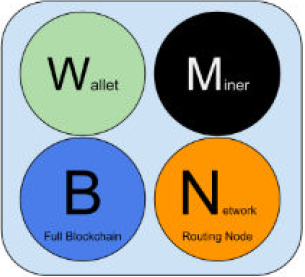
\includegraphics[width=4cm]{imagenes/introduccion/nodo_bitcoin}
    \caption{Un nodo de red bitcoin con las cuatro funciones}
    \label{fig:funciones-nodo}
\end{figure}

\noindent Todos los nodos incluyen funciones de enrutamiento, validan y propagan transacciones y bloques. Los nodos 
completos, también mantienen una copia completa y actualizada de la Blockchain. Se encargan también de verificar de 
forma autónoma y autorizada cualquier transacción sin referencia externa. Los nodos cartera pueden ser parte de un
nodo completo, en este caso suele ser un cliente de bitcoin de escritorio.

\vspace{5mm}

\noindent Algunos nodos mantienen sólo un subconjunto de la cadena de bloque y verifican las transacciones mediante un 
método llamado verificación de pago simplificado. Estos nodos se conocen como SPV o nodos de peso ligero.

\vspace{5mm}

\noindent Los nodos mineros compiten para crear nuevos bloques ejecutando hardware especializado para resolver el 
algoritmo de Proof-of-Work. Pueden ser completos o ligeros.

\vspace{5mm}

\noindent Además de los principales tipos de nodos del protocolo P2P de bitcoin, hay servidores y nodos que ejecutan 
otros protocolos, como los protocolos de piscinas mineras especializadas y los protocolos de acceso a clientes ligeros. 

\newpage

\noindent Aquí están los tipos de nodos más comunes en la red extendida de bitcoin:

\begin{figure}[ht!]
    \centering
    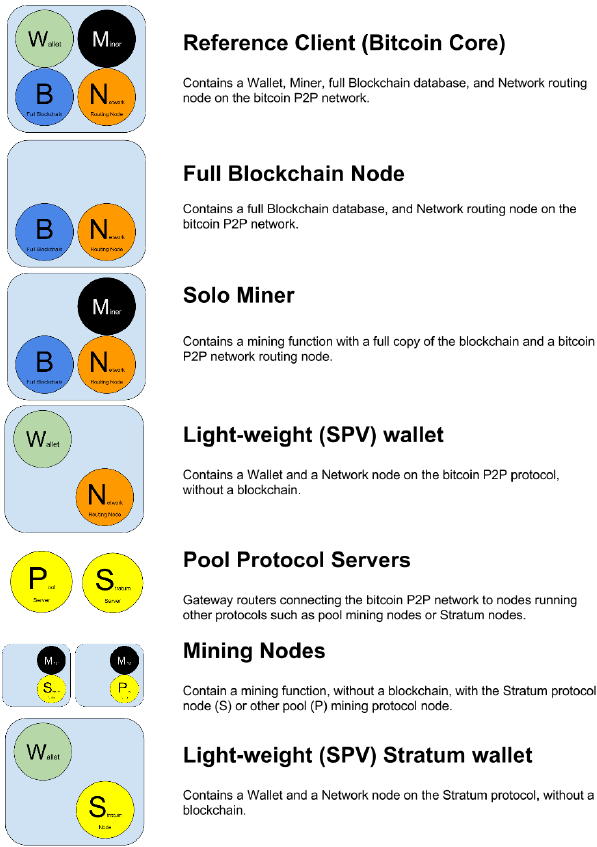
\includegraphics[width=10cm]{imagenes/introduccion/diferentes_nodos_red_extendida}
    \caption{Diferentes tipos de nodos en una red extendida bitcoin}
\end{figure}

\subsubsection{Blockchain}

La tecnología Blockchain, o también conocido como Distributed Ledger Technology, es una lista ordenada de bloques de 
transacciones vinculados hacia atrás. Cada bloque es identificado por un hash, generado por el algoritmo criptográfico 
SHA256, almacenado en la cabecera del bloque. Cada bloque está enlazado con el anterior bloque (bloque padre) a través 
de su hash en la cabecera del bloque. Dicha secuencia, crea una cadena hasta llegar al primer bloque, conocido como 
el bloque génesis.

\vspace{5mm}

\noindent Puede darse el caso de que un bloque tenga varios hijos. Los hijos múltiples surgen cuando se produce un fork 
del Blockchain, se debe a que diferentes bloques son descubiertos casi simultaneamente por diferentes mineros. 
Finalmente, un bloque hijo pasa a formar parte del Blockchain y la división se resuelve. 

\vspace{5mm}

\noindent La DLT es inmutable debido a que, en la cabecera del bloque, contiene el hash del padre y, por lo tanto, 
afecta al bloque actual. La identidad del hijo cambia si la del padre también lo hace. Cuando cambia el padre, el 
hash del padre cambia, y por tanto hay que modificar la cabecera del bloque. Esto a su vez cambia el hash del hijo y 
por tanto requiere un cambio en el puntero del nieto y así sucesivamente.

\vspace{5mm}

\noindent Este efecto de cascada asegura que una vez que un bloque tiene muchas generaciones que lo siguen, no puede 
ser cambiado sin forzar un recálculo de todos los bloques subsiguientes. La existencia de una larga cadena Blockchain 
hace que la historia profunda de la cadena de bloques sea inmutable.

\subsubsection{Minería y consensos}

La minería es la encargada de validar nuevas transacciones, comprobando si son fradulentas, y se registran en el 
libro de contabilidad global. Asimismo, se ocupa de añadir nuevos bitcoins a la oferta monetaria, ya que los 
mineros proporcionan potencia de procesamiento a la red de bitcoin a cambio de la oportunidad de ser recompensados.

\vspace{5mm}

\noindent Cada 10 minutos se \say{extrae} un nuevo bloque que contiene las transacciones que se han producido desde el 
último, añadiendo así esas transacciones a la cadena de bloques. Las transacciones que pasan a formar parte de un bloque 
y se añaden a la cadena de bloques se consideran \say{confirmadas} lo que permite a los nuevos propietarios de bitcoin 
gastar el bitcoin recibido en esas transacciones.

\vspace{5mm}

\noindent Los mineros pueden recibir dos tipos de recompensas: las creadas por nuevos bloques y tasas de transacciones 
de todas las transacciones dentro del bloque. Para ello, tiene que competir entre ellos para encontrar la solución a 
un problema difícil basado en un algoritmo criptográfico de hash. La solución del problema, llamada Proof-of-Work, 
se incluye en el nuevo bloque y actúa como prueba de que el minero gastó un esfuerzo de computación significativo. 
La competencia por resolver el algoritmo de PoW para ganar recompensas y el derecho a registrar las transacciones 
en la cadena de bloques, es la base del modelo de seguridad de Bitcoin.

\vspace{5mm}

\noindent La minería es el principal proceso de la cámara de compensación descentralizada, por el cual las transacciones 
son validadas y autorizadas. La minería asegura el sistema de bitcoin y permite el surgimiento de consenso en toda la 
red sin una autoridad central.

\subsubsection*{Consenso decentralizado}

A diferencia de los sistemas de pagos tradicionales, el Bitcoin no tiene una autoridad central sino que cada nodo tiene
una copia completa de un libro de cuentas público como registro de autoridad. Cada nodo de la red comparte la 
información transmitida y, en conclusión, ensamblará una copia del mismo libro público de todos los demás.

\vspace{5mm}

\noindent El consenso descentralizado de Bitcoin surge de la interacción de cuatro procesos que se producen de forma 
independiente en los nodos de la red:

\begin{itemize}
    \item Verificación independiente de cada transacción, por cada nodo completo, sobre la base de una lista completa 
    de criterios
    \item La agregación independiente de esas transacciones en nuevos bloques por nodos mineros, junto con un cálculo 
    demostrado a través de un algoritmo de prueba de trabajo
    \item Verificación independiente de los nuevos bloques por cada nodo y ensamblaje en una cadena
    \item Selección independiente, por cada nodo, de la cadena con el cálculo más acumulativo demostrado a través del 
    PoW
\end{itemize}

\subsubsection*{Algoritmo Proof-of-Work}

La idea de PoW fue publicada por primera vez en 1993 por Cynthia Dwork y Moni Naor, y posteriormente fue 
aplicada por Satoshi Nakamoto en el Bitcoin en 2008. 

\vspace{5mm}

\noindent El problema matemático se puede describir de forma abstracta de la siguiente forma: 

\vspace{5mm}

\noindent \textit{Dados los datos A, encuentra un número x como el que el hash de x adjunto a los resultados de A es un 
número menor que el de B.}

\vspace{5mm}

\noindent La respuesta al problema debe ser un número menor que el hash del bloque para que sea aceptado, conocido como 
el \say{hash del objetivo}. Un hash del objetivo es un número que el encabezamiento de un bloque de hash debe ser igual 
o menor que el de un nuevo bloque, junto con la recompensa, para ser otorgado a un minero. Cuanto más bajo es un 
objetivo, más difícil es generar un bloque.

\vspace{5mm}

\noindent El consenso de prueba de trabajo más utilizado se basa en el SHA-256 y se introdujo como parte de Bitcoin.

\vspace{5mm}

\noindent Características del algoritmo: 

\begin{itemize}
    \item Es difícil encontrar una solución para el problema matemático
    \item Es fácil verificar la corrección de esa solución
\end{itemize}

\subsection{Internet de las Cosas (IoT)}

El Internet de las Cosas, o también conocido cómo Internet of Things, consiste en dispositivos que generan procesos, e 
intercambian grandes cantidades de información a través de Internet. Recolectan y comparten datos sobre cómo son 
utilizados y sobre el medio que los rodea. Esta información puede ser utilizada para detertar patrones, hacer 
recomendaciones y detectar posibles problemas antes de que ocurran.

\vspace{5mm}

\noindent Desde usos personales como zapatos inteligentes para proveer apoyo al seguimiento y análisis de los datos de 
actitud física, como servicios a la comunidad: control de la cirugía en los hospitales, detectar condiciones 
meteorológicas y proporcionar rastreo y conectividad en los automóviles.

\vspace{5mm}

\noindent  Los objetos y sistemas inteligentes permiten automatizar ciertas tareas, especialmente cuando éstas son 
repetitivas, mundanas, requieren mucho tiempo o incluso son peligrosas.

\subsection{La seguridad del Blockchain en IoT}

El uso de la tecnología Blockchain dentro del ambito de los dispositivos IoT, ha tomado un papel importante en la 
gestión, control y seguridad. En esta sección, vamos a describir como la tecnología Blockchain puede ser clave para
proporcionr soluciones de seguridad a los problemas actuales del Internet de las Cosas.

\begin{itemize}
    \item \textbf{Espacio de direcciones}: Blockchain tiene 160-bit de espacio de direcciones, a diferencia de IPv6
    que solo tiene 128-bit. Esto es debido a que el hash de la clave pública generada por ECDSA (Elliptic Cruve Digital
    Algorithm) es de 20 bytes o 160-bits. Por lo tanto, podemos alojar alrededor de \(1,46*10^{48}\) direcciones para 
    dispositivos IoT. Lo que hace que sea más escalable a diferencia de IPv6. 
    \item \textbf{Identidad y administración}: Blockchain tiene la capacidad de resolver estos desafíos de manera fácil, 
    segura y eficiente. Se ha utilizado ampliamente para proporcionar un registro de identidad fiable y autorizado, 
    el seguimiento de la propiedad y la supervisión de productos, bienes y activos.
    \item \textbf{Autenticación e integridad de los datos}: Por su diseño, los datos transmitidos siempre estarán
    criptográficamente probados y firmados, garantizando así la autenticación e integridad de los datos.
    \item \textbf{Autenticación, autorización y privacidad}: Provee una solución efectiva en autorización, privacidad en
    los datos y la habilidad de suminstrar reglas de autenticación decentralizada. 
    \item \textbf{Comunicaciones seguras}: Los protocolos que utilizan las IoT son HTTP, MQTT, CoAP o XMPP, y no son 
    seguros por diseño y por tanto, son envueltos por una capa DTLS o TLS. Con Blockchain, la gestión y distribución 
    de claves se elimina totalmente, y cada dispositivo IoT tendrá su par de claves simétricas, para conectarse a la 
    Blockchain.
\end{itemize}

\subsection{¿Qué es una Raspberry Pi?}

La Rasberry Pi es un ordenador de bajo coste hecho por la Raspberry Pi Foundation, del tamaño de una tarjeta de crédito, 
permite aprender programación, construir proyectos de hardware, hacer automatización del hogar, e incluso a nivel 
industrial. Además, tiene la capacidad de interactuar con el mundo exterior, y se ha utilizado en una amplia gama de 
proyectos de creación digital, desde máquinas de música hasta estaciones meteorológicas.

\vspace{5mm}

\noindent El primer modelo lanzado al mercado, tenía una CPU de un solo núcleo de 700MHz y 256MB de RAM, hasta hoy en 
día que tenemos el modelo 4 con Quad core de 1.5GHz y con diferentes versiones de 2GB, 4GB y 8GB DDR4 de RAM.

\vspace{5mm}

\noindent Aunque existen diferentes alternativas, hemos utilizado la Rasberry Pi para este proyecto por comodidad, ya 
que he podido trabajar antes con diferentes modelos de la marca.

\subsection{Conclusión}

En este capítulo hemos dado una introducción al proyecto. Hemos hablado sobre la tecnología Blockchain, apoyandonos 
con el concepto de Bitcoin. Para pasar ha comentar sobre el Internet de las Cosas, y su combinación con el Blockchain, 
También hemos comentado sobre los dispositivos que voy a utilizar como prueba de concepto. A continuación, indagararemos 
más sobre otras tecnologías que han aplicado el Blockchain y plataformas.

\newpage
\section{Herramientas para el desarrollo blockchain}

\subsection{Tipos de redes Blockchain}

\subsection{Plataformas Blockchain}

\subsection{Smart Contracts}

https://blockchainhub.net/smart-contracts/

\subsection{Herramientas utilizadas para Hyperledger Fabric}

\subsection{Herramientas utilizadas para desarrollo del proyecto}

\subsection{La seguridad del Blockchain en IoT}

\newpage
\section{Sistema propuesto.}

En esta sección vamos a exponer los requisitos extraidos del análisis de la descripción del proyecto, que se van a 
especificar en los requisitos funcionales y no funcionales, los caso de uso, sus actores y diagramas de clase y secuencia.
Se comentará sobre la arquitectura que se ha elaborado para la prueba de concepto y qué planificación y presupuesto se
ha llevado a cabo.

\subsection{Análisis de requerimientos.}

\subsubsection{Requisitos funcionales.}

\paragraph{RF-1. Gestión de usuarios.} Habrá dos actores principales: los usuarios finales y el administrador.

\begin{itemize}
    \item[] RF-1.1. El usuario podrá solicitar darse de alta.
    \item[] RF-1.2. El usuario podrá solicitar darse de baja.
    \item[] RF-1.3. El administrador podrá dar de alta a un usuario en la red Blockchain.
    \item[] RF-1.4. El administrador podrá revocar el certificado de un usuario en la red Blockchain.
    \item[] RF-1.5. El administrador podrá renovar el certificado de un usuario en la red Blockchain.
\end{itemize}

\paragraph{RF-2. Gestión de dispositivos.} El sistema permitirá la gestión de dispositivos IoT de los usuarios, dentro de 
la aplicación. Podemos catalogar los dispositivos entre: sensores y actuadores.

\begin{itemize}
    \item[] RF-2.1. El usuario tendrá permitido añadir un dispositivo indicando un nombre, su número serial y su dirección
    IP.
    \item[] RF-2.2. El usuario podrá establecer un valor númerico al sensor como valor de entrada y se comprobará las 
    condiciones de sus enlaces en el cual se encuentre involucrado.
    \item[] RF-2.3. El usuario no podrá establecer un valor númerico al actuador, se dejará por defecto el -1.
    \item[] RF-2.4. El usuario podrá borrar el dispositivo de la red, indicando el número serial.
    \item[] RF-2.5. El usuario podrá consultar todos los dispositivos añadidos a la aplicación.
    \item[] RF-2.6. El usuario podrá consultar los datos del dispositivo indicando el número serial.
    \item[] RF-2.7. El usuario podrá consultar el historial de un dispositivos indicando el número serial.
\end{itemize}

\paragraph{RF-3. Gestión de enlaces.} El sistema permitirá la gestión de enlaces de dispositivos IoT dentro de la 
aplicación. Los enlaces  viene a representar la relación que hay entre un sensor y un actuador, mediante una condición de 
activación.

\begin{itemize}
    \item[] RF-3.1. El usuario tendrá permitido añadir un enlace indicando los dispositivos que lo forman (el número 
    serial del sensor y el número serial del actuador), la región donde se encuentre los dispositivo, y una condición, 
    formada por una variable, acompañado de un operador de comparación y un valor númerico. Al añadirse, tendrá su estado 
    activado por defecto.
    \item[] RF-3.2. El usuario podrá actualizar un enlace, indicando su ID (hash del número serial del sensor y el 
    actuador). Podrá cambiar la condición y la región.
    \item[] RF-3.3. El usuario podrá borrar un enlace, indicando su ID.
    \item[] RF-3.4. El usuario podrá habilitar un enlace, y se mandará una señal de activación al actuador. 
    \item[] RF-3.5. El usuario podrá deshabilitar un enlace, y se mandará una señal de desactivación al actuador.
    \item[] RF-3.6. El usuario podrá consultar todos los enlaces añadidos a la aplicación.
    \item[] RF-3.6. El usuario podrá consultar los datos del enlace indicando el ID del mismo.
    \item[] RF-3.7. El usuario podrá consultar el historial de un enlace indicando el ID del mismo.
\end{itemize}

\subsubsection{Requisitos no funcionales.}

\begin{itemize}
    \item[] RNF-1. La aplicación ha de ser accesible desde fuera de la red local, con cualquier dispositivo, smartphone, 
    table, portatil o sobremesa
    \item[] RNF-2. La aplicación tiene que ser compatible con diferentes navegadores.
    \item[] RNF-3. Se establecerán conexiones seguras dentro de la aplicación, cifrando las peticiones HTTP.
    \item[] RNF-4. La aplicación tiene que cumplir los criterios de PWA, tiene que trabajar de forma offline, mandar
    notificaciones y soportar la sincronización en segundo plano.
    \item[] RNF-5. La aplicación tiene que adaptarse a cualquier dimension de pantalla, es decir, tiene que ser responsive.
    \item[] RNF-6. La aplicación tiene que cumplir niveles de rendimiento, accesibilidad y SEO\footnote{ SEO significa 
    Search Engine Optimization (optimización de motores de búsqueda), que es la práctica de aumentar la cantidad y la 
    calidad del tráfico se un sitio web a través de los resultados orgánicos de los motores de búsqueda \cite{what-is-seo}. 
    \label{fnlabel}} aceptables, utilizando la aplicación LightHouse\footnote{ Es una herramienta elaborada por Google de 
    código abierto para mejorar la calidad de las páginas web \cite{lighthouse}. \label{fnlabel}}.
    \item[] RNF-7. La interfaz ha de ser clara e intuitiva.
    \item[] RNF-8. Se realizarán test a la aplicación.
    \item[] RNF-8. No se requerirá de conocimientos previos para el uso de la aplicación.
    \item[] RNF-9. La API tiene que ser accesible desde la aplicación, para realizar cualquier petición directamente
    a la red Blockchain.
\end{itemize}

\subsection{Especificación.}

\subsubsection{Actores de los casos de uso.}

\begin{itemize}
    \item \textbf{Entorno}: es el actor vinculado al medio ambiente, se incluye lo referente al aire, la temperatura, la humedad,
    el tiempo atmosférico, etc. Los sensores se van a encargar de recoger eso datos del exterior y manejarlos.
    \item \textbf{Dispositivo}: es el actor que realiza un mecanismo con una función específica. Podemos diferenciar entre sensores
    y actuadores.
    \item \textbf{Usuario}: es el actor que puede usar las principales funcionalidades que ofrece la aplicación una vez que 
    tenga un certificado de autoridad dentro de la red Blockchain. Podrá llevar una gestión de sus dispositivos y enlaces dentro
    de la aplicación y gracias a la tecnología Blockchain, podrá ver toda la trazabilidad de las transacciones realizadas y 
    resistente a modificaciones.
    \item \textbf{Administrador}: es el actor encargado de la gestión de usuarios, se encargará de administrar todo lo relacionado
    con los certificados de autoridad de cada usuario del sistema.
\end{itemize}

\subsubsection{Especificación de casos de uso.}

\begin{itemize}
    \item Caso de uso 1: Solicitar dar de alta a un usuario.
    
    \begin{table}[h!]
        \centering
        \begin{tabular}{|l|p{0.753\textwidth}|}
            \hline
            \textbf{Casos de Uso}   &   Dar de alta a un usuario (CU\_01). \\
            \hline 
            \textbf{Actores}        &   Usuario (Principal) y Administrador (Secundario). \\ 
            \hline 
            \textbf{Tipo}           &   Primario y esencial. \\
            \hline
            \textbf{Referencias}    &   RF-1.1., RF-1.3. \\ 
            \hline
            \textbf{Precondición}   &   El usuario no debe de tener un certificado de autoridad asociada en la red. \\ 
            \hline
            \textbf{Postcondición}  &   El usuario tendrá un certificado de autoridad. \\ 
            \hline
        \end{tabular}
        
        \vspace{5mm}
        
        \begin{tabular}{|p{\textwidth}|}
            \hline
            \rowcolor{SeaGreen} \textbf{Propósito} \\
            \hline
            \multicolumn{1}{|p{12cm}|}{El usuario obtendrá el certificado de autoridad para poder realizar operaciones en el sistema, firmando las 
            transacciones.} \\ [0.5ex]
            \hline
        \end{tabular}
        
        \vspace{5mm}
        
        \begin{tabular}{|p{\textwidth}|}
            \hline
            \rowcolor{SeaGreen} \textbf{Resumen} \\
            \hline
            \multicolumn{1}{|p{12cm}|}{El usuario solicitará al administrador la petición de darse de alta del sistem. El administrador se encargará de 
            crear el certificado de autoridad del usuario y lo guardará en la cartera, para que el usuario pueda realizar acciones en la 
            aplicación.} \\ [0.5ex]
            \hline
        \end{tabular}
        
        \vspace{5mm}
        
        \begin{tabular}{|p{0.01\textwidth}|p{0.438\textwidth}|p{0.01\textwidth}|p{0.438\textwidth}|}
            \cline{1-4}
            \rowcolor{SeaGreen} \multicolumn{4}{|l|}{\textbf{Curso Normal}} \\
            \cline{1-4}
            \textbf{1} & Usuario: manda petición de darse de alta. & & \\
            \hline
            \textbf{2} & Administrador: manda petición para crear el certificado de autoridad. & & \\
            \hline
             & & \textbf{3} & El sistema crea el certificado de autoridad. \\
            \hline
             & & \textbf{4} & El sistema guarda el certificado en la cartera (wallet). \\
            \hline
        \end{tabular}
        
        \vspace{5mm}
        
        \begin{tabular}{|p{0.224\textwidth}|p{0.224\textwidth}|p{0.224\textwidth}|p{0.224\textwidth}|}
            \cline{1-4}
            \rowcolor{SeaGreen} \multicolumn{4}{|l|}{\textbf{Otros datos}} \\
            \cline{1-4}
            \textbf{Frecuencia \newline esperada} & Media & \textbf{Rendimiento} &  \\
            \hline
            \textbf{Importancia} & Alta & \textbf{Urgencia} & Alta \\
            \hline
            \textbf{Estado} & & \textbf{Estabilidad} & Alta \\
            \hline
        \end{tabular}
        
        \caption{Caso de uso 1: Dar de alta a un usuario.}
        \label{table:caso-de-uso-1}
    \end{table}
    
    \newpage
    
    \item Caso de uso 2: Solicitar dar de baja a un usuario. 
    
    \begin{table}[h!]
        \centering
        \begin{tabular}{|l|p{0.753\textwidth}|}
            \hline
            \textbf{Casos de Uso}   &   Dar de baja a un usuario (CU\_02). \\
            \hline 
            \textbf{Actores}        &   Usuario (Principal) y Administrador (Secundario). \\ 
            \hline 
            \textbf{Tipo}           &   Primario y esencial. \\
            \hline
            \textbf{Referencias}    &   RF-1.2., RF-1.4.\\ 
            \hline
            \textbf{Precondición}   &   El usuario debe de tener un certificado de autoridad asociada en la red.\\ 
            \hline
            \textbf{Postcondición}  &   El usuario no tendra un certificado de autoridad.\\ 
            \hline
        \end{tabular}
        
        \vspace{5mm}
        
        \begin{tabular}{|p{\textwidth}|}
            \hline
            \rowcolor{SeaGreen} \textbf{Propósito} \\
            \hline
            \multicolumn{1}{|p{12cm}|}{El usuario perderá el certificado de autoridad y por tanto no podrá realizar
            ninguna operación en la red.} \\ [0.5ex]
            \hline
        \end{tabular}
        
        \vspace{5mm}
        
        \begin{tabular}{|p{\textwidth}|}
            \hline
            \rowcolor{SeaGreen} \textbf{Resumen} \\
            \hline
            \multicolumn{1}{|p{12cm}|}{El usuario solicitará al administrador la petición de darse de baja del sistema. El administrador
            se encargará de revocar el certificado de autoridad del usuario. El certificado de autoridad se borrará de la cartera (wallet).} \\ [0.5ex]
            \hline
        \end{tabular}
        
        \vspace{5mm}
        
        \begin{tabular}{|p{0.01\textwidth}|p{0.438\textwidth}|p{0.01\textwidth}|p{0.438\textwidth}|}
            \cline{1-4}
            \rowcolor{SeaGreen} \multicolumn{4}{|l|}{\textbf{Curso Normal}} \\
            \cline{1-4}
            \textbf{1} & Usuario: manda petición de darse de baja. & & \\
            \hline
            \textbf{2} & Administrador: manda petición para revocar el certificado de autoridad. & & \\
            \hline
             & & \textbf{3} & El sistema revoca el certificado de autoridad. \\
            \hline
             & & \textbf{4} & El sistema borra el certificado de la cartera (wallet). \\
            \hline
        \end{tabular}
        
        \vspace{5mm}
        
        \begin{tabular}{|p{0.224\textwidth}|p{0.224\textwidth}|p{0.224\textwidth}|p{0.224\textwidth}|}
            \cline{1-4}
            \rowcolor{SeaGreen} \multicolumn{4}{|l|}{\textbf{Otros datos}} \\
            \cline{1-4}
            \textbf{Frecuencia \newline esperada} & Media & \textbf{Rendimiento} &  \\
            \hline
            \textbf{Importancia} & Alta & \textbf{Urgencia} & Alta \\
            \hline
            \textbf{Estado} & & \textbf{Estabilidad} & Alta \\
            \hline
        \end{tabular}
        
        \caption{Caso de uso 2: Solicitar dar de baja a un usuario.}
        \label{table:caso-de-uso-2}
    \end{table}

    \newpage

    \item Caso de uso 3: Dar de alta a un usuario. 
    
    \begin{table}[h!]
        \centering
        \begin{tabular}{|l|p{0.753\textwidth}|}
            \hline
            \textbf{Casos de Uso}   &   Dar de alta a un usuario (CU\_03). \\
            \hline 
            \textbf{Actores}        &   Administrador (Principal) y Usuario (Secundario)\\ 
            \hline 
            \textbf{Tipo}           &   Primario y esencial. \\ 
            \hline
            \textbf{Referencias}    &   RF-1.3., RF-1.1. \\ 
            \hline
            \textbf{Precondición}   &   El Administrador debe de recibir una solicitud de dar de alta. \\ 
            \hline
            \textbf{Postcondición}  &   El certificado de autoridad se guarda en el sistema. \\ 
            \hline
        \end{tabular}
        
        \vspace{5mm}
        
        \begin{tabular}{|p{\textwidth}|}
            \hline
            \rowcolor{SeaGreen} \textbf{Propósito} \\
            \hline
            \multicolumn{1}{|p{12cm}|}{El administrador mandará la solicitud al sistema, para crear el certificado de autoridad.} \\ [0.5ex]
            \hline
        \end{tabular}
        
        \vspace{5mm}
        
        \begin{tabular}{|p{\textwidth}|}
            \hline
            \rowcolor{SeaGreen} \textbf{Resumen} \\
            \hline
            \multicolumn{1}{|p{12cm}|}{El administrador se encargará de crear el certificado de autoridad del usuario y
            lo guardará en la cartera, para que el usuario pueda realizar acciones en la aplicación.} \\ [0.5ex]
            \hline
        \end{tabular}
        
        \vspace{5mm}
        
        \begin{tabular}{|p{0.01\textwidth}|p{0.438\textwidth}|p{0.01\textwidth}|p{0.438\textwidth}|}
            \cline{1-4}
            \rowcolor{SeaGreen} \multicolumn{4}{|l|}{\textbf{Curso Normal}} \\
            \cline{1-4}
            \textbf{1} & Administrador: manda petición para crear el certificado de autoridad. &  &  \\
            \hline
             & & \textbf{2} & El sistema crea el certificado de autoridad. \\
            \hline
             & & \textbf{3} & El sistema guarda el certificado en la cartera (wallet). \\
            \hline
        \end{tabular}
        
        \vspace{5mm}
        
        \begin{tabular}{|p{0.224\textwidth}|p{0.224\textwidth}|p{0.224\textwidth}|p{0.224\textwidth}|}
            \cline{1-4}
            \rowcolor{SeaGreen} \multicolumn{4}{|l|}{\textbf{Otros datos}} \\
            \cline{1-4}
            \textbf{Frecuencia \newline esperada} & Media & \textbf{Rendimiento} &  \\
            \hline
            \textbf{Importancia} & Alta & \textbf{Urgencia} & Alta \\
            \hline
            \textbf{Estado} & & \textbf{Estabilidad} & Alta \\
            \hline
        \end{tabular}
        
        \caption{Caso de uso 3: Dar de alta a un usuario.}
        \label{table:caso-de-uso-3}
    \end{table}
    
    \newpage
    
    \item Caso de uso 4: Dar de baja a un usuario.
    
    \begin{table}[h!]
        \centering
        \begin{tabular}{|l|p{0.753\textwidth}|}
            \hline
            \textbf{Casos de Uso}   &   Dar de baja a un usuario (CU\_04). \\
            \hline 
            \textbf{Actores}        &   Administrador (Principal) y Usuario (Secundario). \\ 
            \hline 
            \textbf{Tipo}           &   Primario y esencial. \\ 
            \hline
            \textbf{Referencias}    &   RF-1.4., RF-1.2.\\ 
            \hline
            \textbf{Precondición}   &   Debe de existir un certificado de autoridad asociado al usuario.\\ 
            \hline
            \textbf{Postcondición}  &   Se revoca el certificado.\\ 
            \hline
        \end{tabular}
        
        \vspace{5mm}
        
        \begin{tabular}{|p{\textwidth}|}
            \hline
            \rowcolor{SeaGreen} \textbf{Propósito} \\
            \hline
            \multicolumn{1}{|p{12cm}|}{El administrador mandará la solicitud al sistema, para revocar el certificado
            de autoridad del usuario.} \\ [0.5ex]
            \hline
        \end{tabular}
        
        \vspace{5mm}
        
        \begin{tabular}{|p{\textwidth}|}
            \hline
            \rowcolor{SeaGreen} \textbf{Resumen} \\
            \hline
            \multicolumn{1}{|p{12cm}|}{El administrador se encargará de revocar el certificado de autoridad del usuario.
            El certificado de autoridad se borrará de la cartera (wallet).} \\ [0.5ex]
            \hline
        \end{tabular}
        
        \vspace{5mm}
        
        \begin{tabular}{|p{0.01\textwidth}|p{0.438\textwidth}|p{0.01\textwidth}|p{0.438\textwidth}|}
            \cline{1-4}
            \rowcolor{SeaGreen} \multicolumn{4}{|l|}{\textbf{Curso Normal}} \\
            \cline{1-4}
            \textbf{1} & Administrador: manda petición para revocar el certificado de autoridad. &  &  \\
            \hline
             & & \textbf{2} & El sistema revoca el certificado de autoridad. \\
            \hline
             & & \textbf{3} & El sistema borra el certificado de autoridad de la carter (wallet). \\
            \hline
        \end{tabular}
        
        \vspace{5mm}
        
        \begin{tabular}{|p{0.224\textwidth}|p{0.224\textwidth}|p{0.224\textwidth}|p{0.224\textwidth}|}
            \cline{1-4}
            \rowcolor{SeaGreen} \multicolumn{4}{|l|}{\textbf{Otros datos}} \\
            \cline{1-4}
            \textbf{Frecuencia \newline esperada} & Media & \textbf{Rendimiento} &  \\
            \hline
            \textbf{Importancia} & Alta & \textbf{Urgencia} & Alta \\
            \hline
            \textbf{Estado} & & \textbf{Estabilidad} & Alta \\
            \hline
        \end{tabular}
        
        \caption{Caso de uso 4: Dar de baja a un usuario.}
        \label{table:caso-de-uso-4}
    \end{table}
    
    \newpage

    \item Caso de uso 5: Renovar el certificado de autoridad del usuario.
    
    \begin{table}[h!]
        \centering
        \begin{tabular}{|l|p{0.753\textwidth}|}
            \hline
            \textbf{Casos de Uso}   &   Renovar el certificado de autoridad del usuario (CU\_05). \\
            \hline 
            \textbf{Actores}        &   Administrador (Principal) y Usuario (Secundario). \\ 
            \hline 
            \textbf{Tipo}           &   Primario y esencial. \\ 
            \hline
            \textbf{Referencias}    &   RF-1.5., RF-1.4.\\ 
            \hline
            \textbf{Precondición}   &  Debe de existir un certificado de autoridad asociado al usuario y tiene que 
            haber expirado la fecha de finalización del certificado. \\ 
            \hline
            \textbf{Postcondición}  &  Se emite un nuevo certificado de autoridad para el usuario. \\ 
            \hline
        \end{tabular}
        
        \vspace{5mm}
        
        \begin{tabular}{|p{\textwidth}|}
            \hline
            \rowcolor{SeaGreen} \textbf{Propósito} \\
            \hline
            \multicolumn{1}{|p{12cm}|}{El administrador mandará la solicitud al sistema, para renovar el 
            certificado de autoridad del usuario.} \\ [0.5ex]
            \hline
        \end{tabular}
        
        \vspace{5mm}
        
        \begin{tabular}{|p{\textwidth}|}
            \hline
            \rowcolor{SeaGreen} \textbf{Resumen} \\
            \hline
            \multicolumn{1}{|p{12cm}|}{El administrado manda la petición de renovación, que consiste en la emisión de un nuevo 
            certificado para que el sistema (CA) extienda la vida útil de la misma más allá de la fecha de finalización del certificado
            original.} \\ [0.5ex]
            \hline
        \end{tabular}
        
        \vspace{5mm}
        
        \begin{tabular}{|p{0.01\textwidth}|p{0.438\textwidth}|p{0.01\textwidth}|p{0.438\textwidth}|}
            \cline{1-4}
            \rowcolor{SeaGreen} \multicolumn{4}{|l|}{\textbf{Curso Normal}} \\
            \cline{1-4}
            \textbf{1} & Administrador: comprueba la fecha de expiración del certificado. &  &  \\
            \hline
            \textbf{2} & Administrador: manda la petición para renovar el certificado. & & \\
            \hline
             & & \textbf{3} & El sistema renueva el certificado de autoridad. \\
            \hline
             & & \textbf{4} & El sistema guarda el certificado en la cartera (wallet). \\
             \hline
        \end{tabular}
        
        \vspace{5mm}
        
        \begin{tabular}{|p{0.224\textwidth}|p{0.224\textwidth}|p{0.224\textwidth}|p{0.224\textwidth}|}
            \cline{1-4}
            \rowcolor{SeaGreen} \multicolumn{4}{|l|}{\textbf{Otros datos}} \\
            \cline{1-4}
            \textbf{Frecuencia \newline esperada} & Media & \textbf{Rendimiento} & Alta \\
            \hline
            \textbf{Importancia} & Alta & \textbf{Urgencia} & Media \\
            \hline
            \textbf{Estado} & & \textbf{Estabilidad} & Alta \\
            \hline
        \end{tabular}
        
        \caption{Caso de uso 5: Renovar el certificado de autoridad del usuario.}
        \label{table:caso-de-uso-5}
    \end{table}
    
    \newpage
    
    \item Caso de uso 6: Añadir un dispositivo.
    
    \begin{table}[h!]
        \centering
        \begin{tabular}{|l|p{0.753\textwidth}|}
            \hline
            \textbf{Casos de Uso}   &   Añadir un dispositivo (CU\_06). \\
            \hline 
            \textbf{Actores}        &   Dispositivo (Principal). \\ 
            \hline 
            \textbf{Tipo}           &   Primario y esencial. \\ 
            \hline
            \textbf{Referencias}    &   RF-2.1. \\ 
            \hline
            \textbf{Precondición}   &   No debe de existir un dispositivo con el mismo número serial o direccón IP en el sistema. \\ 
            \hline
            \textbf{Postcondición}  &   Se añade el nuevo dispositivo con valor -1. \\ 
            \hline
        \end{tabular}
        
        \vspace{5mm}
        
        \begin{tabular}{|p{\textwidth}|}
            \hline
            \rowcolor{SeaGreen} \textbf{Propósito} \\
            \hline
            \multicolumn{1}{|p{12cm}|}{El usuario podrá añadir un dispositivo que no esté registrado anteriormente.} \\ [0.5ex]
            \hline
        \end{tabular}
        
        \vspace{5mm}
        
        \begin{tabular}{|p{\textwidth}|}
            \hline
            \rowcolor{SeaGreen} \textbf{Resumen} \\
            \hline
            \multicolumn{1}{|p{12cm}|}{El usuario introducirá los datos asociados con el dispositivo, que son el nombre, el número serial 
            y la dirección IP. Se comprobará que no haya un dispositivo existente con el número serial y la dirección IP iguales, en ese 
            caso se añadirá el dispositivo con el atributo valor -1 por defecto.} \\ [0.5ex]
            \hline
        \end{tabular}
        
        \vspace{5mm}
        
        \begin{tabular}{|p{0.01\textwidth}|p{0.438\textwidth}|p{0.01\textwidth}|p{0.438\textwidth}|}
            \cline{1-4}
            \rowcolor{SeaGreen} \multicolumn{4}{|l|}{\textbf{Curso Normal}} \\
            \cline{1-4}
            \textbf{1} & Usuario: introducirá los datos del dispositivo. &  &  \\
            \hline
             & & \textbf{2} & El sistema comprueba los datos introducidos. \\
            \hline
             & & \textbf{3} & El sistema valida los datos y guarda el nuevo dispositivo en la red Blockchain. \\
            \hline
        \end{tabular}
        
        \vspace{5mm}
        
        \begin{tabular}{|p{0.224\textwidth}|p{0.224\textwidth}|p{0.224\textwidth}|p{0.224\textwidth}|}
            \cline{1-4}
            \rowcolor{SeaGreen} \multicolumn{4}{|l|}{\textbf{Otros datos}} \\
            \cline{1-4}
            \textbf{Frecuencia \newline esperada} & Alta & \textbf{Rendimiento} & Media \\
            \hline
            \textbf{Importancia} & Media & \textbf{Urgencia} & Baja \\
            \hline
            \textbf{Estado} & & \textbf{Estabilidad} & Alta \\
            \hline
        \end{tabular}
        
        \caption{Caso de uso 6: Añadir un dispositivo.}
        \label{table:caso-de-uso-6}
    \end{table}
    
    \newpage

    \item Caso de uso 7: Modificar el valor de entrada de un sensor.
    
    \begin{table}[h!]
        \centering
        \begin{tabular}{|l|p{0.753\textwidth}|}
            \hline
            \textbf{Casos de Uso}   &   Modificar el valor de entrada de un sensor (CU\_07). \\
            \hline 
            \textbf{Actores}        &   Dispositivo (Principal), Entorno (Secundario) y Usuario (Secundario). \\ 
            \hline 
            \textbf{Tipo}           &   Primario y esencial. \\ 
            \hline
            \textbf{Referencias}    &       \\ 
            \hline
            \textbf{Precondición}   &       \\ 
            \hline
            \textbf{Postcondición}  &       \\ 
            \hline
        \end{tabular}
        
        \vspace{5mm}
        
        \begin{tabular}{|p{\textwidth}|}
            \hline
            \rowcolor{SeaGreen} \textbf{Propósito} \\
            \hline
            \multicolumn{1}{|p{12cm}|}{} \\ [0.5ex]
            \hline
        \end{tabular}
        
        \vspace{5mm}
        
        \begin{tabular}{|p{\textwidth}|}
            \hline
            \rowcolor{SeaGreen} \textbf{Resumen} \\
            \hline
            \multicolumn{1}{|p{12cm}|}{} \\ [0.5ex]
            \hline
        \end{tabular}
        
        \vspace{5mm}
        
        \begin{tabular}{|p{0.01\textwidth}|p{0.438\textwidth}|p{0.01\textwidth}|p{0.438\textwidth}|}
            \cline{1-4}
            \rowcolor{SeaGreen} \multicolumn{4}{|l|}{\textbf{Curso Normal}} \\
            \cline{1-4}
            \textbf{1} & Actor1: Acción realizada por el actor &  &  \\
            \hline
            \textbf{2} & Actor1: Acción realizada por el actor & \textbf{3} & Acción realizada por el sistema \\
            \hline
             & & & \\
            \hline
        \end{tabular}
        
        \vspace{5mm}
        
        \begin{tabular}{|p{0.224\textwidth}|p{0.224\textwidth}|p{0.224\textwidth}|p{0.224\textwidth}|}
            \cline{1-4}
            \rowcolor{SeaGreen} \multicolumn{4}{|l|}{\textbf{Otros datos}} \\
            \cline{1-4}
            \textbf{Frecuencia \newline esperada} &  & \textbf{Rendimiento} &  \\
            \hline
            \textbf{Importancia} & & \textbf{Urgencia} & \\
            \hline
            \textbf{Estado} & & \textbf{Estabilidad} & \\
            \hline
        \end{tabular}
        
        \caption{Caso de uso 7: Modificar el valor de entrada de un sensor.}
        \label{table:caso-de-uso-7}
    \end{table}
    
    \newpage
    
    \item Caso de uso 8: 
    
    \begin{table}[h!]
        \centering
        \begin{tabular}{|l|p{0.753\textwidth}|}
            \hline
            \textbf{Casos de Uso}   &   (CU\_08). \\
            \hline 
            \textbf{Actores}        &       \\ 
            \hline 
            \textbf{Tipo}           &   Primario y esencial. \\ 
            \hline
            \textbf{Referencias}    &       \\ 
            \hline
            \textbf{Precondición}   &       \\ 
            \hline
            \textbf{Postcondición}  &       \\ 
            \hline
        \end{tabular}
        
        \vspace{5mm}
        
        \begin{tabular}{|p{\textwidth}|}
            \hline
            \rowcolor{SeaGreen} \textbf{Propósito} \\
            \hline
            \multicolumn{1}{|p{12cm}|}{} \\ [0.5ex]
            \hline
        \end{tabular}
        
        \vspace{5mm}
        
        \begin{tabular}{|p{\textwidth}|}
            \hline
            \rowcolor{SeaGreen} \textbf{Resumen} \\
            \hline
            \multicolumn{1}{|p{12cm}|}{} \\ [0.5ex]
            \hline
        \end{tabular}
        
        \vspace{5mm}
        
        \begin{tabular}{|p{0.01\textwidth}|p{0.438\textwidth}|p{0.01\textwidth}|p{0.438\textwidth}|}
            \cline{1-4}
            \rowcolor{SeaGreen} \multicolumn{4}{|l|}{\textbf{Curso Normal}} \\
            \cline{1-4}
            \textbf{1} & Actor1: Acción realizada por el actor &  &  \\
            \hline
            \textbf{2} & Actor1: Acción realizada por el actor & \textbf{3} & Acción realizada por el sistema \\
            \hline
             & & & \\
            \hline
        \end{tabular}
        
        \vspace{5mm}
        
        \begin{tabular}{|p{0.224\textwidth}|p{0.224\textwidth}|p{0.224\textwidth}|p{0.224\textwidth}|}
            \cline{1-4}
            \rowcolor{SeaGreen} \multicolumn{4}{|l|}{\textbf{Otros datos}} \\
            \cline{1-4}
            \textbf{Frecuencia \newline esperada} &  & \textbf{Rendimiento} &  \\
            \hline
            \textbf{Importancia} & & \textbf{Urgencia} & \\
            \hline
            \textbf{Estado} & & \textbf{Estabilidad} & \\
            \hline
        \end{tabular}
        
        \caption{Caso de uso 8:}
        \label{table:caso-de-uso-8}
    \end{table}
    
    \newpage

    \item Caso de uso 9: 
    
    \begin{table}[h!]
        \centering
        \begin{tabular}{|l|p{0.753\textwidth}|}
            \hline
            \textbf{Casos de Uso}   &   (CU\_09). \\
            \hline 
            \textbf{Actores}        &       \\ 
            \hline 
            \textbf{Tipo}           &   Primario y esencial. \\ 
            \hline
            \textbf{Referencias}    &       \\ 
            \hline
            \textbf{Precondición}   &       \\ 
            \hline
            \textbf{Postcondición}  &       \\ 
            \hline
        \end{tabular}
        
        \vspace{5mm}
        
        \begin{tabular}{|p{\textwidth}|}
            \hline
            \rowcolor{SeaGreen} \textbf{Propósito} \\
            \hline
            \multicolumn{1}{|p{12cm}|}{} \\ [0.5ex]
            \hline
        \end{tabular}
        
        \vspace{5mm}
        
        \begin{tabular}{|p{\textwidth}|}
            \hline
            \rowcolor{SeaGreen} \textbf{Resumen} \\
            \hline
            \multicolumn{1}{|p{12cm}|}{} \\ [0.5ex]
            \hline
        \end{tabular}
        
        \vspace{5mm}
        
        \begin{tabular}{|p{0.01\textwidth}|p{0.438\textwidth}|p{0.01\textwidth}|p{0.438\textwidth}|}
            \cline{1-4}
            \rowcolor{SeaGreen} \multicolumn{4}{|l|}{\textbf{Curso Normal}} \\
            \cline{1-4}
            \textbf{1} & Actor1: Acción realizada por el actor &  &  \\
            \hline
            \textbf{2} & Actor1: Acción realizada por el actor & \textbf{3} & Acción realizada por el sistema \\
            \hline
             & & & \\
            \hline
        \end{tabular}
        
        \vspace{5mm}
        
        \begin{tabular}{|p{0.01\textwidth}|p{.954\textwidth}|}
            \cline{1-2}
            \rowcolor{SeaGreen} \multicolumn{2}{|l|}{\textbf{Cursos Alternos}} \\
            \cline{1-2}
             &  \\
            \hline
             &  \\
            \hline
        \end{tabular}
        
        \vspace{5mm}
        
        \begin{tabular}{|p{0.224\textwidth}|p{0.224\textwidth}|p{0.224\textwidth}|p{0.224\textwidth}|}
            \cline{1-4}
            \rowcolor{SeaGreen} \multicolumn{4}{|l|}{\textbf{Otros datos}} \\
            \cline{1-4}
            \textbf{Frecuencia \newline esperada} &  & \textbf{Rendimiento} &  \\
            \hline
            \textbf{Importancia} & & \textbf{Urgencia} & \\
            \hline
            \textbf{Estado} & & \textbf{Estabilidad} & \\
            \hline
        \end{tabular}
        
        \caption{Caso de uso 9:}
        \label{table:caso-de-uso-9}
    \end{table}
    
    \newpage
    
    \item Caso de uso 10: 
    
    \begin{table}[h!]
        \centering
        \begin{tabular}{|l|p{0.753\textwidth}|}
            \hline
            \textbf{Casos de Uso}   &   (CU\_10). \\
            \hline 
            \textbf{Actores}        &       \\ 
            \hline 
            \textbf{Tipo}           &   Primario y esencial. \\ 
            \hline
            \textbf{Referencias}    &       \\ 
            \hline
            \textbf{Precondición}   &       \\ 
            \hline
            \textbf{Postcondición}  &       \\ 
            \hline
        \end{tabular}
        
        \vspace{5mm}
        
        \begin{tabular}{|p{\textwidth}|}
            \hline
            \rowcolor{SeaGreen} \textbf{Propósito} \\
            \hline
            \multicolumn{1}{|p{12cm}|}{} \\ [0.5ex]
            \hline
        \end{tabular}
        
        \vspace{5mm}
        
        \begin{tabular}{|p{\textwidth}|}
            \hline
            \rowcolor{SeaGreen} \textbf{Resumen} \\
            \hline
            \multicolumn{1}{|p{12cm}|}{} \\ [0.5ex]
            \hline
        \end{tabular}
        
        \vspace{5mm}
        
        \begin{tabular}{|p{0.01\textwidth}|p{0.438\textwidth}|p{0.01\textwidth}|p{0.438\textwidth}|}
            \cline{1-4}
            \rowcolor{SeaGreen} \multicolumn{4}{|l|}{\textbf{Curso Normal}} \\
            \cline{1-4}
            \textbf{1} & Actor1: Acción realizada por el actor &  &  \\
            \hline
            \textbf{2} & Actor1: Acción realizada por el actor & \textbf{3} & Acción realizada por el sistema \\
            \hline
             & & & \\
            \hline
        \end{tabular}
        
        \vspace{5mm}
        
        \begin{tabular}{|p{0.224\textwidth}|p{0.224\textwidth}|p{0.224\textwidth}|p{0.224\textwidth}|}
            \cline{1-4}
            \rowcolor{SeaGreen} \multicolumn{4}{|l|}{\textbf{Otros datos}} \\
            \cline{1-4}
            \textbf{Frecuencia \newline esperada} &  & \textbf{Rendimiento} &  \\
            \hline
            \textbf{Importancia} & & \textbf{Urgencia} & \\
            \hline
            \textbf{Estado} & & \textbf{Estabilidad} & \\
            \hline
        \end{tabular}
        
        \caption{Caso de uso 10:}
        \label{table:caso-de-uso-10}
    \end{table}
    
    \newpage

    \item Caso de uso 11: 
    
    \begin{table}[h!]
        \centering
        \begin{tabular}{|l|p{0.753\textwidth}|}
            \hline
            \textbf{Casos de Uso}   &   (CU\_11). \\
            \hline 
            \textbf{Actores}        &       \\ 
            \hline 
            \textbf{Tipo}           &   Primario y esencial. \\
            \hline
            \textbf{Referencias}    &       \\ 
            \hline
            \textbf{Precondición}   &       \\ 
            \hline
            \textbf{Postcondición}  &       \\ 
            \hline
        \end{tabular}
        
        \vspace{5mm}
        
        \begin{tabular}{|p{\textwidth}|}
            \hline
            \rowcolor{SeaGreen} \textbf{Propósito} \\
            \hline
            \multicolumn{1}{|p{12cm}|}{} \\ [0.5ex]
            \hline
        \end{tabular}
        
        \vspace{5mm}
        
        \begin{tabular}{|p{\textwidth}|}
            \hline
            \rowcolor{SeaGreen} \textbf{Resumen} \\
            \hline
            \multicolumn{1}{|p{12cm}|}{} \\ [0.5ex]
            \hline
        \end{tabular}
        
        \vspace{5mm}
        
        \begin{tabular}{|p{0.01\textwidth}|p{0.438\textwidth}|p{0.01\textwidth}|p{0.438\textwidth}|}
            \cline{1-4}
            \rowcolor{SeaGreen} \multicolumn{4}{|l|}{\textbf{Curso Normal}} \\
            \cline{1-4}
            \textbf{1} & Actor1: Acción realizada por el actor &  &  \\
            \hline
            \textbf{2} & Actor1: Acción realizada por el actor & \textbf{3} & Acción realizada por el sistema \\
            \hline
             & & & \\
            \hline
        \end{tabular}
        
        \vspace{5mm}
        
        \begin{tabular}{|p{0.224\textwidth}|p{0.224\textwidth}|p{0.224\textwidth}|p{0.224\textwidth}|}
            \cline{1-4}
            \rowcolor{SeaGreen} \multicolumn{4}{|l|}{\textbf{Otros datos}} \\
            \cline{1-4}
            \textbf{Frecuencia \newline esperada} &  & \textbf{Rendimiento} &  \\
            \hline
            \textbf{Importancia} & & \textbf{Urgencia} & \\
            \hline
            \textbf{Estado} & & \textbf{Estabilidad} & \\
            \hline
        \end{tabular}
        
        \caption{Caso de uso 11:}
        \label{table:caso-de-uso-11}
    \end{table}
    
    \newpage
    
    \item Caso de uso 12: 
    
    \begin{table}[h!]
        \centering
        \begin{tabular}{|l|p{0.753\textwidth}|}
            \hline
            \textbf{Casos de Uso}   &   (CU\_12). \\
            \hline 
            \textbf{Actores}        &       \\ 
            \hline 
            \textbf{Tipo}           &   Primario y esencial. \\ 
            \hline
            \textbf{Referencias}    &       \\ 
            \hline
            \textbf{Precondición}   &       \\ 
            \hline
            \textbf{Postcondición}  &       \\ 
            \hline
        \end{tabular}
        
        \vspace{5mm}
        
        \begin{tabular}{|p{\textwidth}|}
            \hline
            \rowcolor{SeaGreen} \textbf{Propósito} \\
            \hline
            \multicolumn{1}{|p{12cm}|}{} \\ [0.5ex]
            \hline
        \end{tabular}
        
        \vspace{5mm}
        
        \begin{tabular}{|p{\textwidth}|}
            \hline
            \rowcolor{SeaGreen} \textbf{Resumen} \\
            \hline
            \multicolumn{1}{|p{12cm}|}{} \\ [0.5ex]
            \hline
        \end{tabular}
        
        \vspace{5mm}
        
        \begin{tabular}{|p{0.01\textwidth}|p{0.438\textwidth}|p{0.01\textwidth}|p{0.438\textwidth}|}
            \cline{1-4}
            \rowcolor{SeaGreen} \multicolumn{4}{|l|}{\textbf{Curso Normal}} \\
            \cline{1-4}
            \textbf{1} & Actor1: Acción realizada por el actor &  &  \\
            \hline
            \textbf{2} & Actor1: Acción realizada por el actor & \textbf{3} & Acción realizada por el sistema \\
            \hline
             & & & \\
            \hline
        \end{tabular}
        
        \vspace{5mm}
        
        \begin{tabular}{|p{0.224\textwidth}|p{0.224\textwidth}|p{0.224\textwidth}|p{0.224\textwidth}|}
            \cline{1-4}
            \rowcolor{SeaGreen} \multicolumn{4}{|l|}{\textbf{Otros datos}} \\
            \cline{1-4}
            \textbf{Frecuencia \newline esperada} &  & \textbf{Rendimiento} &  \\
            \hline
            \textbf{Importancia} & & \textbf{Urgencia} & \\
            \hline
            \textbf{Estado} & & \textbf{Estabilidad} & \\
            \hline
        \end{tabular}
        
        \caption{Caso de uso 12:}
        \label{table:caso-de-uso-12}
    \end{table}
    
    \newpage

    \item Caso de uso 13: 
    
    \begin{table}[h!]
        \centering
        \begin{tabular}{|l|p{0.753\textwidth}|}
            \hline
            \textbf{Casos de Uso}   &   (CU\_13). \\
            \hline 
            \textbf{Actores}        &       \\ 
            \hline 
            \textbf{Tipo}           &   Primario y esencial. \\
            \hline
            \textbf{Referencias}    &       \\ 
            \hline
            \textbf{Precondición}   &       \\ 
            \hline
            \textbf{Postcondición}  &       \\ 
            \hline
        \end{tabular}
        
        \vspace{5mm}
        
        \begin{tabular}{|p{\textwidth}|}
            \hline
            \rowcolor{SeaGreen} \textbf{Propósito} \\
            \hline
            \multicolumn{1}{|p{12cm}|}{} \\ [0.5ex]
            \hline
        \end{tabular}
        
        \vspace{5mm}
        
        \begin{tabular}{|p{\textwidth}|}
            \hline
            \rowcolor{SeaGreen} \textbf{Resumen} \\
            \hline
            \multicolumn{1}{|p{12cm}|}{} \\ [0.5ex]
            \hline
        \end{tabular}
        
        \vspace{5mm}
        
        \begin{tabular}{|p{0.01\textwidth}|p{0.438\textwidth}|p{0.01\textwidth}|p{0.438\textwidth}|}
            \cline{1-4}
            \rowcolor{SeaGreen} \multicolumn{4}{|l|}{\textbf{Curso Normal}} \\
            \cline{1-4}
            \textbf{1} & Actor1: Acción realizada por el actor &  &  \\
            \hline
            \textbf{2} & Actor1: Acción realizada por el actor & \textbf{3} & Acción realizada por el sistema \\
            \hline
             & & & \\
            \hline
        \end{tabular}
        
        \vspace{5mm}
        
        \begin{tabular}{|p{0.224\textwidth}|p{0.224\textwidth}|p{0.224\textwidth}|p{0.224\textwidth}|}
            \cline{1-4}
            \rowcolor{SeaGreen} \multicolumn{4}{|l|}{\textbf{Otros datos}} \\
            \cline{1-4}
            \textbf{Frecuencia \newline esperada} &  & \textbf{Rendimiento} &  \\
            \hline
            \textbf{Importancia} & & \textbf{Urgencia} & \\
            \hline
            \textbf{Estado} & & \textbf{Estabilidad} & \\
            \hline
        \end{tabular}
        
        \caption{Caso de uso 13:}
        \label{table:caso-de-uso-13}
    \end{table}
    
    \newpage
    
    \item Caso de uso 14: 
    
    \begin{table}[h!]
        \centering
        \begin{tabular}{|l|p{0.753\textwidth}|}
            \hline
            \textbf{Casos de Uso}   &   (CU\_14). \\
            \hline 
            \textbf{Actores}        &       \\ 
            \hline 
            \textbf{Tipo}           &   Primario y esencial. \\ 
            \hline
            \textbf{Referencias}    &       \\ 
            \hline
            \textbf{Precondición}   &       \\ 
            \hline
            \textbf{Postcondición}  &       \\ 
            \hline
        \end{tabular}
        
        \vspace{5mm}
        
        \begin{tabular}{|p{\textwidth}|}
            \hline
            \rowcolor{SeaGreen} \textbf{Propósito} \\
            \hline
            \multicolumn{1}{|p{12cm}|}{} \\ [0.5ex]
            \hline
        \end{tabular}
        
        \vspace{5mm}
        
        \begin{tabular}{|p{\textwidth}|}
            \hline
            \rowcolor{SeaGreen} \textbf{Resumen} \\
            \hline
            \multicolumn{1}{|p{12cm}|}{} \\ [0.5ex]
            \hline
        \end{tabular}
        
        \vspace{5mm}
        
        \begin{tabular}{|p{0.01\textwidth}|p{0.438\textwidth}|p{0.01\textwidth}|p{0.438\textwidth}|}
            \cline{1-4}
            \rowcolor{SeaGreen} \multicolumn{4}{|l|}{\textbf{Curso Normal}} \\
            \cline{1-4}
            \textbf{1} & Actor1: Acción realizada por el actor &  &  \\
            \hline
            \textbf{2} & Actor1: Acción realizada por el actor & \textbf{3} & Acción realizada por el sistema \\
            \hline
             & & & \\
            \hline
        \end{tabular}
        
        \vspace{5mm}
        
        \begin{tabular}{|p{0.224\textwidth}|p{0.224\textwidth}|p{0.224\textwidth}|p{0.224\textwidth}|}
            \cline{1-4}
            \rowcolor{SeaGreen} \multicolumn{4}{|l|}{\textbf{Otros datos}} \\
            \cline{1-4}
            \textbf{Frecuencia \newline esperada} &  & \textbf{Rendimiento} &  \\
            \hline
            \textbf{Importancia} & & \textbf{Urgencia} & \\
            \hline
            \textbf{Estado} & & \textbf{Estabilidad} & \\
            \hline
        \end{tabular}
        
        \caption{Caso de uso 14:}
        \label{table:caso-de-uso-14}
    \end{table}
    
    \newpage

    \item Caso de uso 15: 
    
    \begin{table}[h!]
        \centering
        \begin{tabular}{|l|p{0.753\textwidth}|}
            \hline
            \textbf{Casos de Uso}   &   (CU\_15). \\
            \hline 
            \textbf{Actores}        &       \\ 
            \hline 
            \textbf{Tipo}           &   Primario y esencial. \\
            \hline
            \textbf{Referencias}    &       \\ 
            \hline
            \textbf{Precondición}   &       \\ 
            \hline
            \textbf{Postcondición}  &       \\ 
            \hline
        \end{tabular}
        
        \vspace{5mm}
        
        \begin{tabular}{|p{\textwidth}|}
            \hline
            \rowcolor{SeaGreen} \textbf{Propósito} \\
            \hline
            \multicolumn{1}{|p{12cm}|}{} \\ [0.5ex]
            \hline
        \end{tabular}
        
        \vspace{5mm}
        
        \begin{tabular}{|p{\textwidth}|}
            \hline
            \rowcolor{SeaGreen} \textbf{Resumen} \\
            \hline
            \multicolumn{1}{|p{12cm}|}{} \\ [0.5ex]
            \hline
        \end{tabular}
        
        \vspace{5mm}
        
        \begin{tabular}{|p{0.01\textwidth}|p{0.438\textwidth}|p{0.01\textwidth}|p{0.438\textwidth}|}
            \cline{1-4}
            \rowcolor{SeaGreen} \multicolumn{4}{|l|}{\textbf{Curso Normal}} \\
            \cline{1-4}
            \textbf{1} & Actor1: Acción realizada por el actor &  &  \\
            \hline
            \textbf{2} & Actor1: Acción realizada por el actor & \textbf{3} & Acción realizada por el sistema \\
            \hline
             & & & \\
            \hline
        \end{tabular}
        
        \vspace{5mm}
        
        \begin{tabular}{|p{0.224\textwidth}|p{0.224\textwidth}|p{0.224\textwidth}|p{0.224\textwidth}|}
            \cline{1-4}
            \rowcolor{SeaGreen} \multicolumn{4}{|l|}{\textbf{Otros datos}} \\
            \cline{1-4}
            \textbf{Frecuencia \newline esperada} &  & \textbf{Rendimiento} &  \\
            \hline
            \textbf{Importancia} & & \textbf{Urgencia} & \\
            \hline
            \textbf{Estado} & & \textbf{Estabilidad} & \\
            \hline
        \end{tabular}
        
        \caption{Caso de uso 15:}
        \label{table:caso-de-uso-15}
    \end{table}
    
    \newpage
    
    \item Caso de uso 16: 
    
    \begin{table}[h!]
        \centering
        \begin{tabular}{|l|p{0.753\textwidth}|}
            \hline
            \textbf{Casos de Uso}   &   (CU\_16). \\
            \hline 
            \textbf{Actores}        &       \\ 
            \hline 
            \textbf{Tipo}           &   Primario y esencial. \\ 
            \hline
            \textbf{Referencias}    &       \\ 
            \hline
            \textbf{Precondición}   &       \\ 
            \hline
            \textbf{Postcondición}  &       \\ 
            \hline
        \end{tabular}
        
        \vspace{5mm}
        
        \begin{tabular}{|p{\textwidth}|}
            \hline
            \rowcolor{SeaGreen} \textbf{Propósito} \\
            \hline
            \multicolumn{1}{|p{12cm}|}{} \\ [0.5ex]
            \hline
        \end{tabular}
        
        \vspace{5mm}
        
        \begin{tabular}{|p{\textwidth}|}
            \hline
            \rowcolor{SeaGreen} \textbf{Resumen} \\
            \hline
            \multicolumn{1}{|p{12cm}|}{} \\ [0.5ex]
            \hline
        \end{tabular}
        
        \vspace{5mm}
        
        \begin{tabular}{|p{0.01\textwidth}|p{0.438\textwidth}|p{0.01\textwidth}|p{0.438\textwidth}|}
            \cline{1-4}
            \rowcolor{SeaGreen} \multicolumn{4}{|l|}{\textbf{Curso Normal}} \\
            \cline{1-4}
            \textbf{1} & Actor1: Acción realizada por el actor &  &  \\
            \hline
            \textbf{2} & Actor1: Acción realizada por el actor & \textbf{3} & Acción realizada por el sistema \\
            \hline
             & & & \\
            \hline
        \end{tabular}
        
        \vspace{5mm}
        
        \begin{tabular}{|p{0.224\textwidth}|p{0.224\textwidth}|p{0.224\textwidth}|p{0.224\textwidth}|}
            \cline{1-4}
            \rowcolor{SeaGreen} \multicolumn{4}{|l|}{\textbf{Otros datos}} \\
            \cline{1-4}
            \textbf{Frecuencia \newline esperada} &  & \textbf{Rendimiento} &  \\
            \hline
            \textbf{Importancia} & & \textbf{Urgencia} & \\
            \hline
            \textbf{Estado} & & \textbf{Estabilidad} & \\
            \hline
        \end{tabular}
        
        \caption{Caso de uso 16:}
        \label{table:caso-de-uso-16}
    \end{table}
    
    \newpage

    \item Caso de uso 17: 
    
    \begin{table}[h!]
        \centering
        \begin{tabular}{|l|p{0.753\textwidth}|}
            \hline
            \textbf{Casos de Uso}   &   (CU\_17). \\
            \hline 
            \textbf{Actores}        &       \\ 
            \hline 
            \textbf{Tipo}           &   Primario y esencial. \\
            \hline
            \textbf{Referencias}    &       \\ 
            \hline
            \textbf{Precondición}   &       \\ 
            \hline
            \textbf{Postcondición}  &       \\ 
            \hline
        \end{tabular}
        
        \vspace{5mm}
        
        \begin{tabular}{|p{\textwidth}|}
            \hline
            \rowcolor{SeaGreen} \textbf{Propósito} \\
            \hline
            \multicolumn{1}{|p{12cm}|}{} \\ [0.5ex]
            \hline
        \end{tabular}
        
        \vspace{5mm}
        
        \begin{tabular}{|p{\textwidth}|}
            \hline
            \rowcolor{SeaGreen} \textbf{Resumen} \\
            \hline
            \multicolumn{1}{|p{12cm}|}{} \\ [0.5ex]
            \hline
        \end{tabular}
        
        \vspace{5mm}
        
        \begin{tabular}{|p{0.01\textwidth}|p{0.438\textwidth}|p{0.01\textwidth}|p{0.438\textwidth}|}
            \cline{1-4}
            \rowcolor{SeaGreen} \multicolumn{4}{|l|}{\textbf{Curso Normal}} \\
            \cline{1-4}
            \textbf{1} & Actor1: Acción realizada por el actor &  &  \\
            \hline
            \textbf{2} & Actor1: Acción realizada por el actor & \textbf{3} & Acción realizada por el sistema \\
            \hline
             & & & \\
            \hline
        \end{tabular}
        
        \vspace{5mm}
        
        \begin{tabular}{|p{0.224\textwidth}|p{0.224\textwidth}|p{0.224\textwidth}|p{0.224\textwidth}|}
            \cline{1-4}
            \rowcolor{SeaGreen} \multicolumn{4}{|l|}{\textbf{Otros datos}} \\
            \cline{1-4}
            \textbf{Frecuencia \newline esperada} &  & \textbf{Rendimiento} &  \\
            \hline
            \textbf{Importancia} & & \textbf{Urgencia} & \\
            \hline
            \textbf{Estado} & & \textbf{Estabilidad} & \\
            \hline
        \end{tabular}
        
        \caption{Caso de uso 17:}
        \label{table:caso-de-uso-17}
    \end{table}
    
    \newpage
    
    \item Caso de uso 18: 
    
    \begin{table}[h!]
        \centering
        \begin{tabular}{|l|p{0.753\textwidth}|}
            \hline
            \textbf{Casos de Uso}   &   (CU\_18). \\
            \hline 
            \textbf{Actores}        &       \\ 
            \hline 
            \textbf{Tipo}           &   Primario y esencial. \\ 
            \hline
            \textbf{Referencias}    &       \\ 
            \hline
            \textbf{Precondición}   &       \\ 
            \hline
            \textbf{Postcondición}  &       \\ 
            \hline
        \end{tabular}
        
        \vspace{5mm}
        
        \begin{tabular}{|p{\textwidth}|}
            \hline
            \rowcolor{SeaGreen} \textbf{Propósito} \\
            \hline
            \multicolumn{1}{|p{12cm}|}{} \\ [0.5ex]
            \hline
        \end{tabular}
        
        \vspace{5mm}
        
        \begin{tabular}{|p{\textwidth}|}
            \hline
            \rowcolor{SeaGreen} \textbf{Resumen} \\
            \hline
            \multicolumn{1}{|p{12cm}|}{} \\ [0.5ex]
            \hline
        \end{tabular}
        
        \vspace{5mm}
        
        \begin{tabular}{|p{0.01\textwidth}|p{0.438\textwidth}|p{0.01\textwidth}|p{0.438\textwidth}|}
            \cline{1-4}
            \rowcolor{SeaGreen} \multicolumn{4}{|l|}{\textbf{Curso Normal}} \\
            \cline{1-4}
            \textbf{1} & Actor1: Acción realizada por el actor &  &  \\
            \hline
            \textbf{2} & Actor1: Acción realizada por el actor & \textbf{3} & Acción realizada por el sistema \\
            \hline
             & & & \\
            \hline
        \end{tabular}
        
        \vspace{5mm}
        
        \begin{tabular}{|p{0.224\textwidth}|p{0.224\textwidth}|p{0.224\textwidth}|p{0.224\textwidth}|}
            \cline{1-4}
            \rowcolor{SeaGreen} \multicolumn{4}{|l|}{\textbf{Otros datos}} \\
            \cline{1-4}
            \textbf{Frecuencia \newline esperada} &  & \textbf{Rendimiento} &  \\
            \hline
            \textbf{Importancia} & & \textbf{Urgencia} & \\
            \hline
            \textbf{Estado} & & \textbf{Estabilidad} & \\
            \hline
        \end{tabular}
        
        \caption{Caso de uso 18:}
        \label{table:caso-de-uso-18}
    \end{table}
    
    \newpage

    \item Caso de uso 19: 
    
    \begin{table}[h!]
        \centering
        \begin{tabular}{|l|p{0.753\textwidth}|}
            \hline
            \textbf{Casos de Uso}   &   (CU\_19). \\
            \hline 
            \textbf{Actores}        &       \\ 
            \hline 
            \textbf{Tipo}           &   Primario y esencial. \\
            \hline
            \textbf{Referencias}    &       \\ 
            \hline
            \textbf{Precondición}   &       \\ 
            \hline
            \textbf{Postcondición}  &       \\ 
            \hline
        \end{tabular}
        
        \vspace{5mm}
        
        \begin{tabular}{|p{\textwidth}|}
            \hline
            \rowcolor{SeaGreen} \textbf{Propósito} \\
            \hline
            \multicolumn{1}{|p{12cm}|}{} \\ [0.5ex]
            \hline
        \end{tabular}
        
        \vspace{5mm}
        
        \begin{tabular}{|p{\textwidth}|}
            \hline
            \rowcolor{SeaGreen} \textbf{Resumen} \\
            \hline
            \multicolumn{1}{|p{12cm}|}{} \\ [0.5ex]
            \hline
        \end{tabular}
        
        \vspace{5mm}
        
        \begin{tabular}{|p{0.01\textwidth}|p{0.438\textwidth}|p{0.01\textwidth}|p{0.438\textwidth}|}
            \cline{1-4}
            \rowcolor{SeaGreen} \multicolumn{4}{|l|}{\textbf{Curso Normal}} \\
            \cline{1-4}
            \textbf{1} & Actor1: Acción realizada por el actor &  &  \\
            \hline
            \textbf{2} & Actor1: Acción realizada por el actor & \textbf{3} & Acción realizada por el sistema \\
            \hline
             & & & \\
            \hline
        \end{tabular}
        
        \vspace{5mm}
        
        \begin{tabular}{|p{0.224\textwidth}|p{0.224\textwidth}|p{0.224\textwidth}|p{0.224\textwidth}|}
            \cline{1-4}
            \rowcolor{SeaGreen} \multicolumn{4}{|l|}{\textbf{Otros datos}} \\
            \cline{1-4}
            \textbf{Frecuencia \newline esperada} &  & \textbf{Rendimiento} &  \\
            \hline
            \textbf{Importancia} & & \textbf{Urgencia} & \\
            \hline
            \textbf{Estado} & & \textbf{Estabilidad} & \\
            \hline
        \end{tabular}
        
        \caption{Caso de uso 19:}
        \label{table:caso-de-uso-19}
    \end{table}
\end{itemize}

\subsubsection{Diagramas de casos de uso.}

\subsubsection{Diagramas de clase.}

\subsubsection{Diagramas de secuencia.}

\subsection{Arquitectura de la red Blockchain.}

\subsection{Planificación y Presupuesto del proyecto.}

\subsection{Conclusión.}

\newpage
\section{Desarrollo del sistema.}

En esta sección vamos a dar paso al desarrollo del proyecto, en primer lugar hablaremos sobre la implementación de la red
blockchain en las Raspberry previamente configuradas, para pasar al desarrollo de la API basada en GraphQL con NodeJS y 
posteriormente a la interfaz de usuario con Gatsby y React.  

\subsection{Configuración y creación de la topología de la red.}

\begin{figure}[ht!]
  \centering
  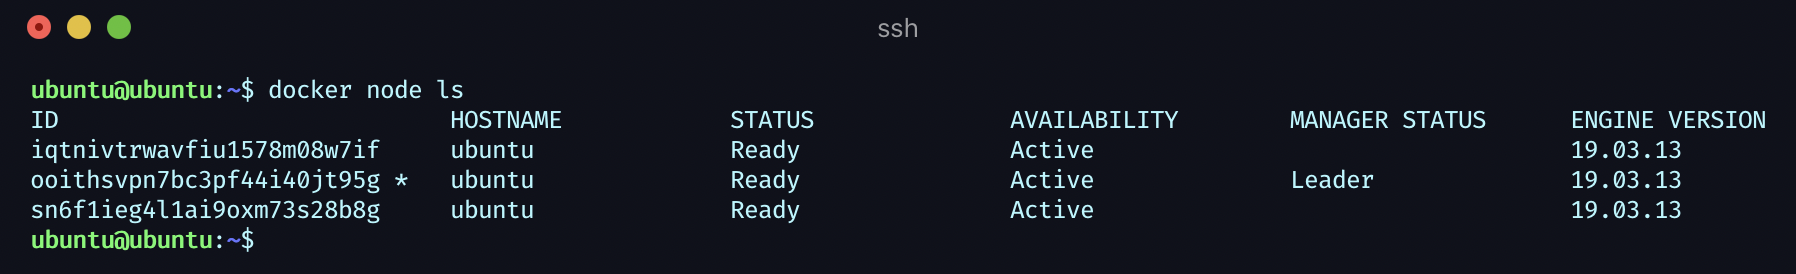
\includegraphics[width=10cm]{imagenes/desarrollo/comandos/node_ls_worker}
  \caption{Nodos de Docker Swarm.}
  \label{fig:node-ls-worker}
\end{figure}

\begin{figure}[ht!]
  \centering
  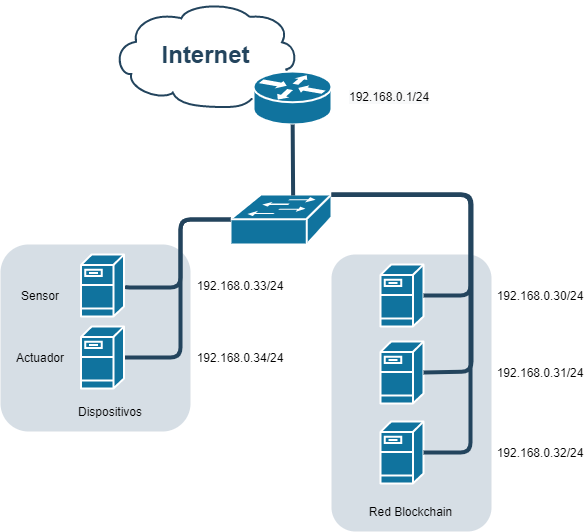
\includegraphics[width=10cm]{imagenes/desarrollo/topologia_red}
  \caption{Topología de la red.}
  \label{fig:topologia-red}
\end{figure}

\begin{figure}[ht!]
  \centering
  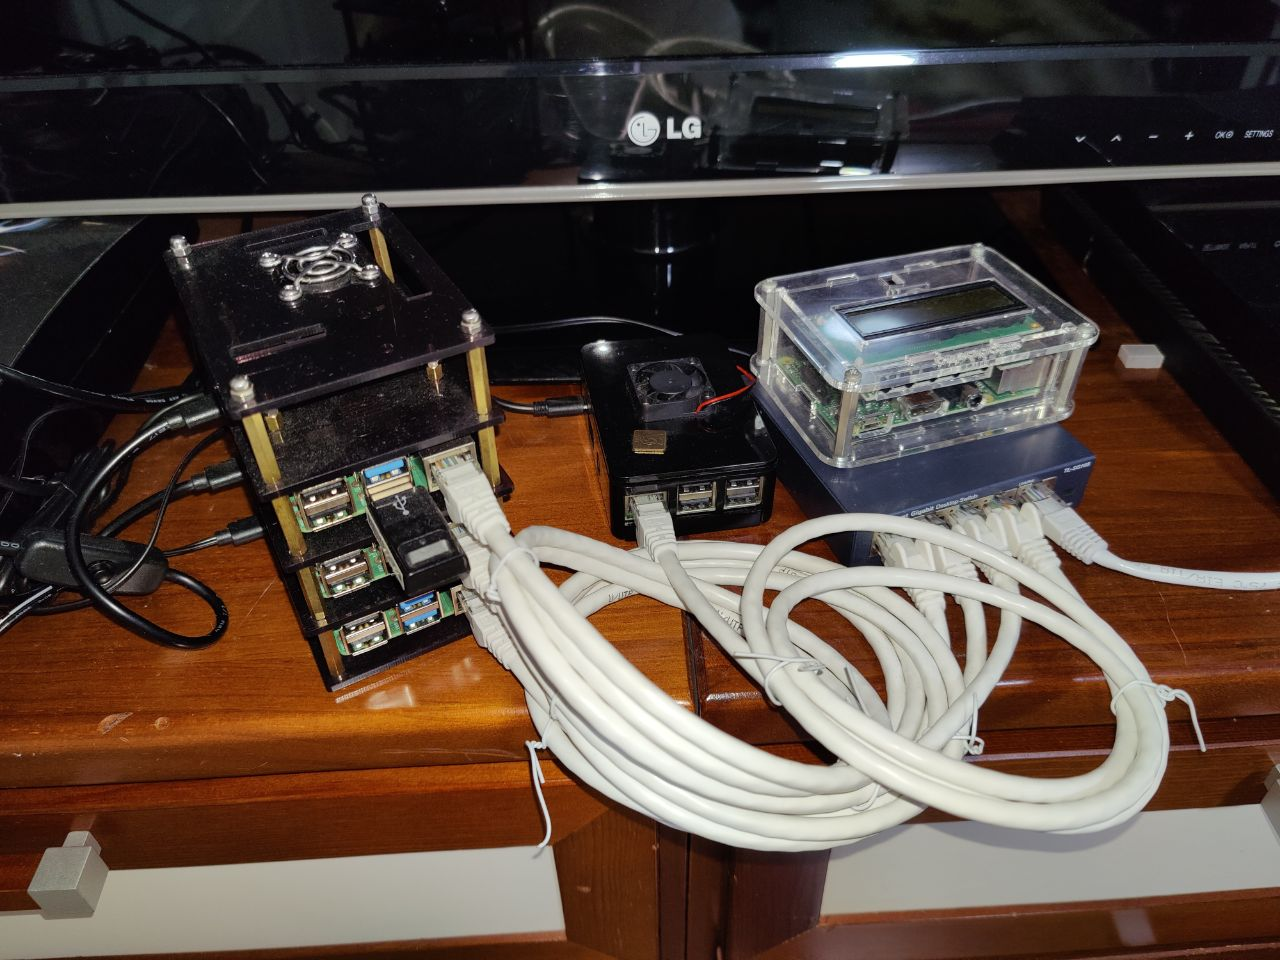
\includegraphics[width=10cm]{imagenes/desarrollo/foto_raspberry}
  \caption{Captura de las Raspberry Pi.}
  \label{fig:captura-raspberry}
\end{figure}

\begin{figure}[ht!]
  \centering
  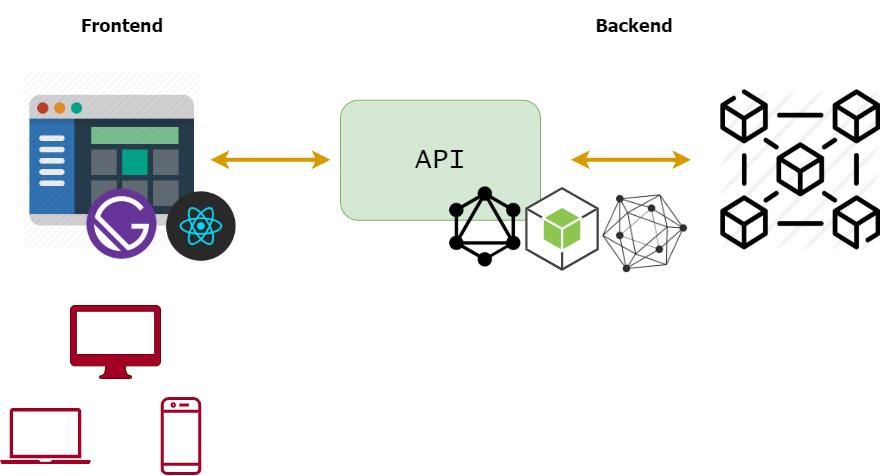
\includegraphics[width=10cm]{imagenes/desarrollo/arquitectura_aplicacion}
  \caption{Arquitectura de la aplicación.}
  \label{fig:arquitectura-aplicacion}
\end{figure}

\subsection{Implementación de la red Blockchain.}

\begin{figure}[ht!]
  \centering
  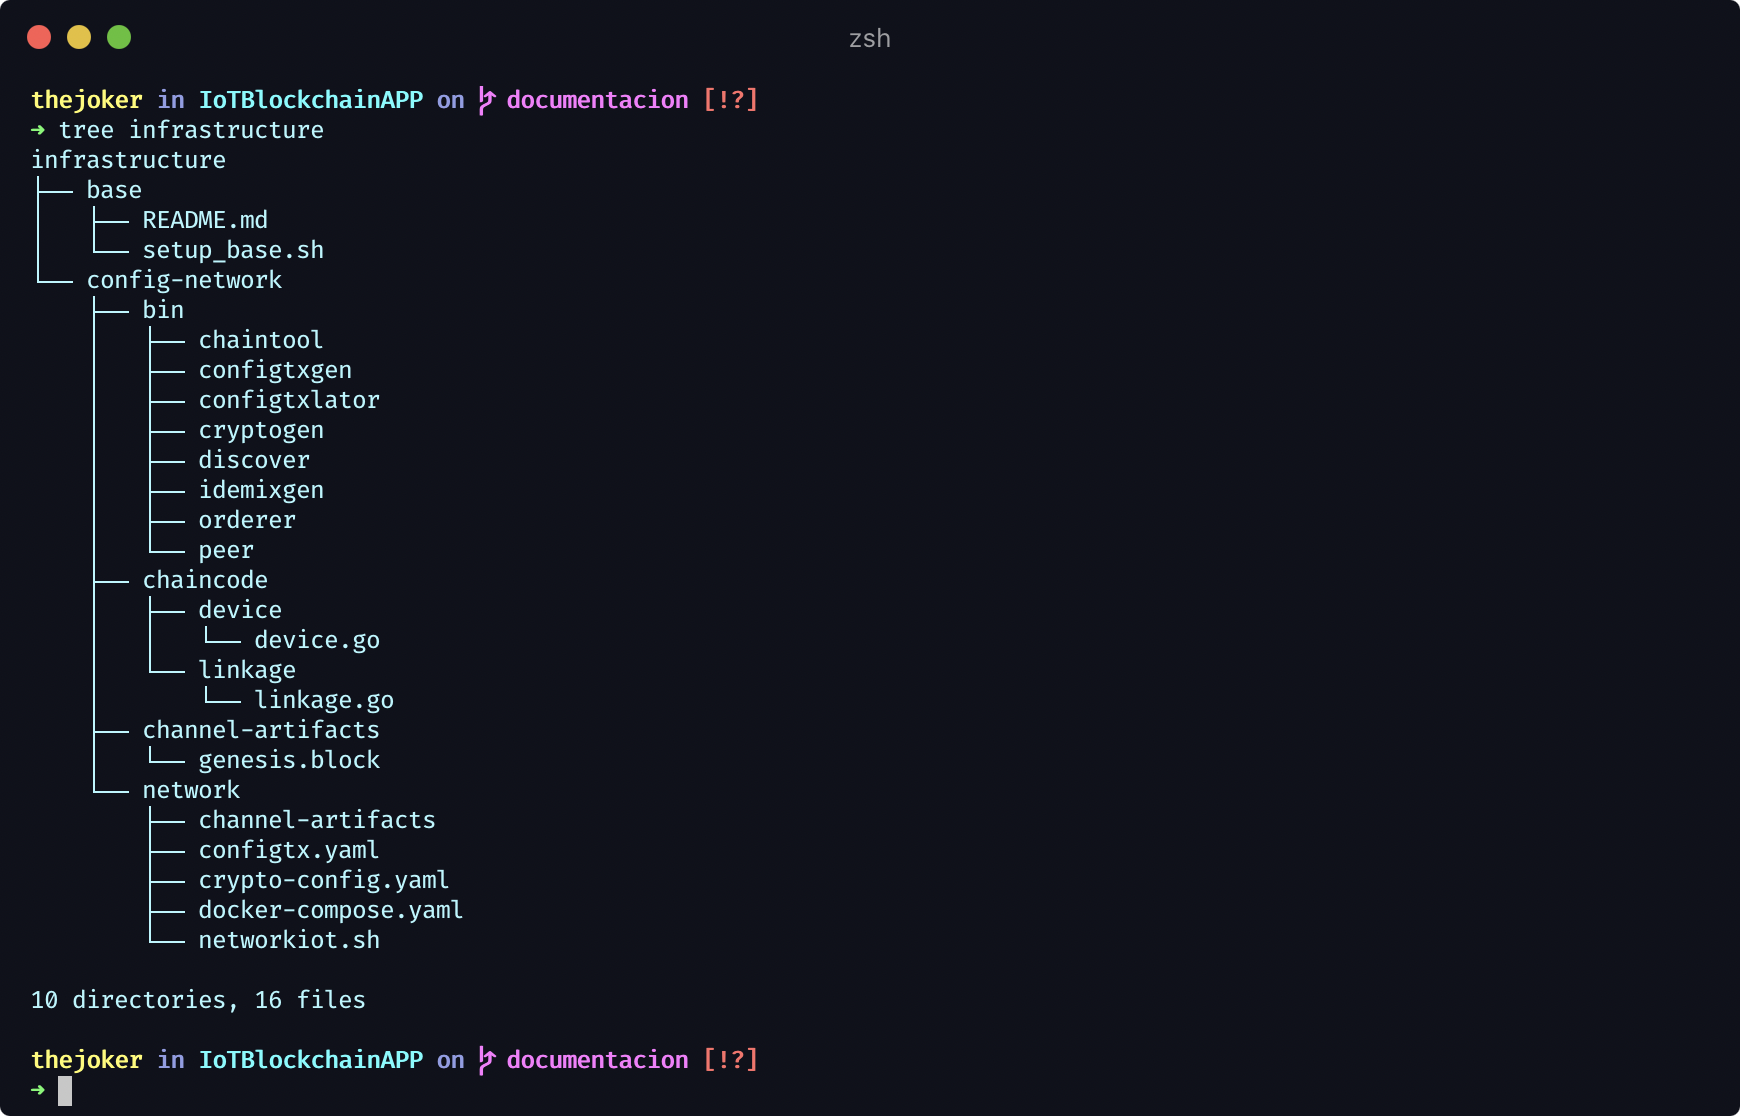
\includegraphics[width=10cm]{imagenes/desarrollo/tree_infraestructure}
  \caption{Tree de la carpeta infraestructure.}
  \label{fig:tree-infraestructure}
\end{figure}

\begin{figure}[ht!]
  \centering
  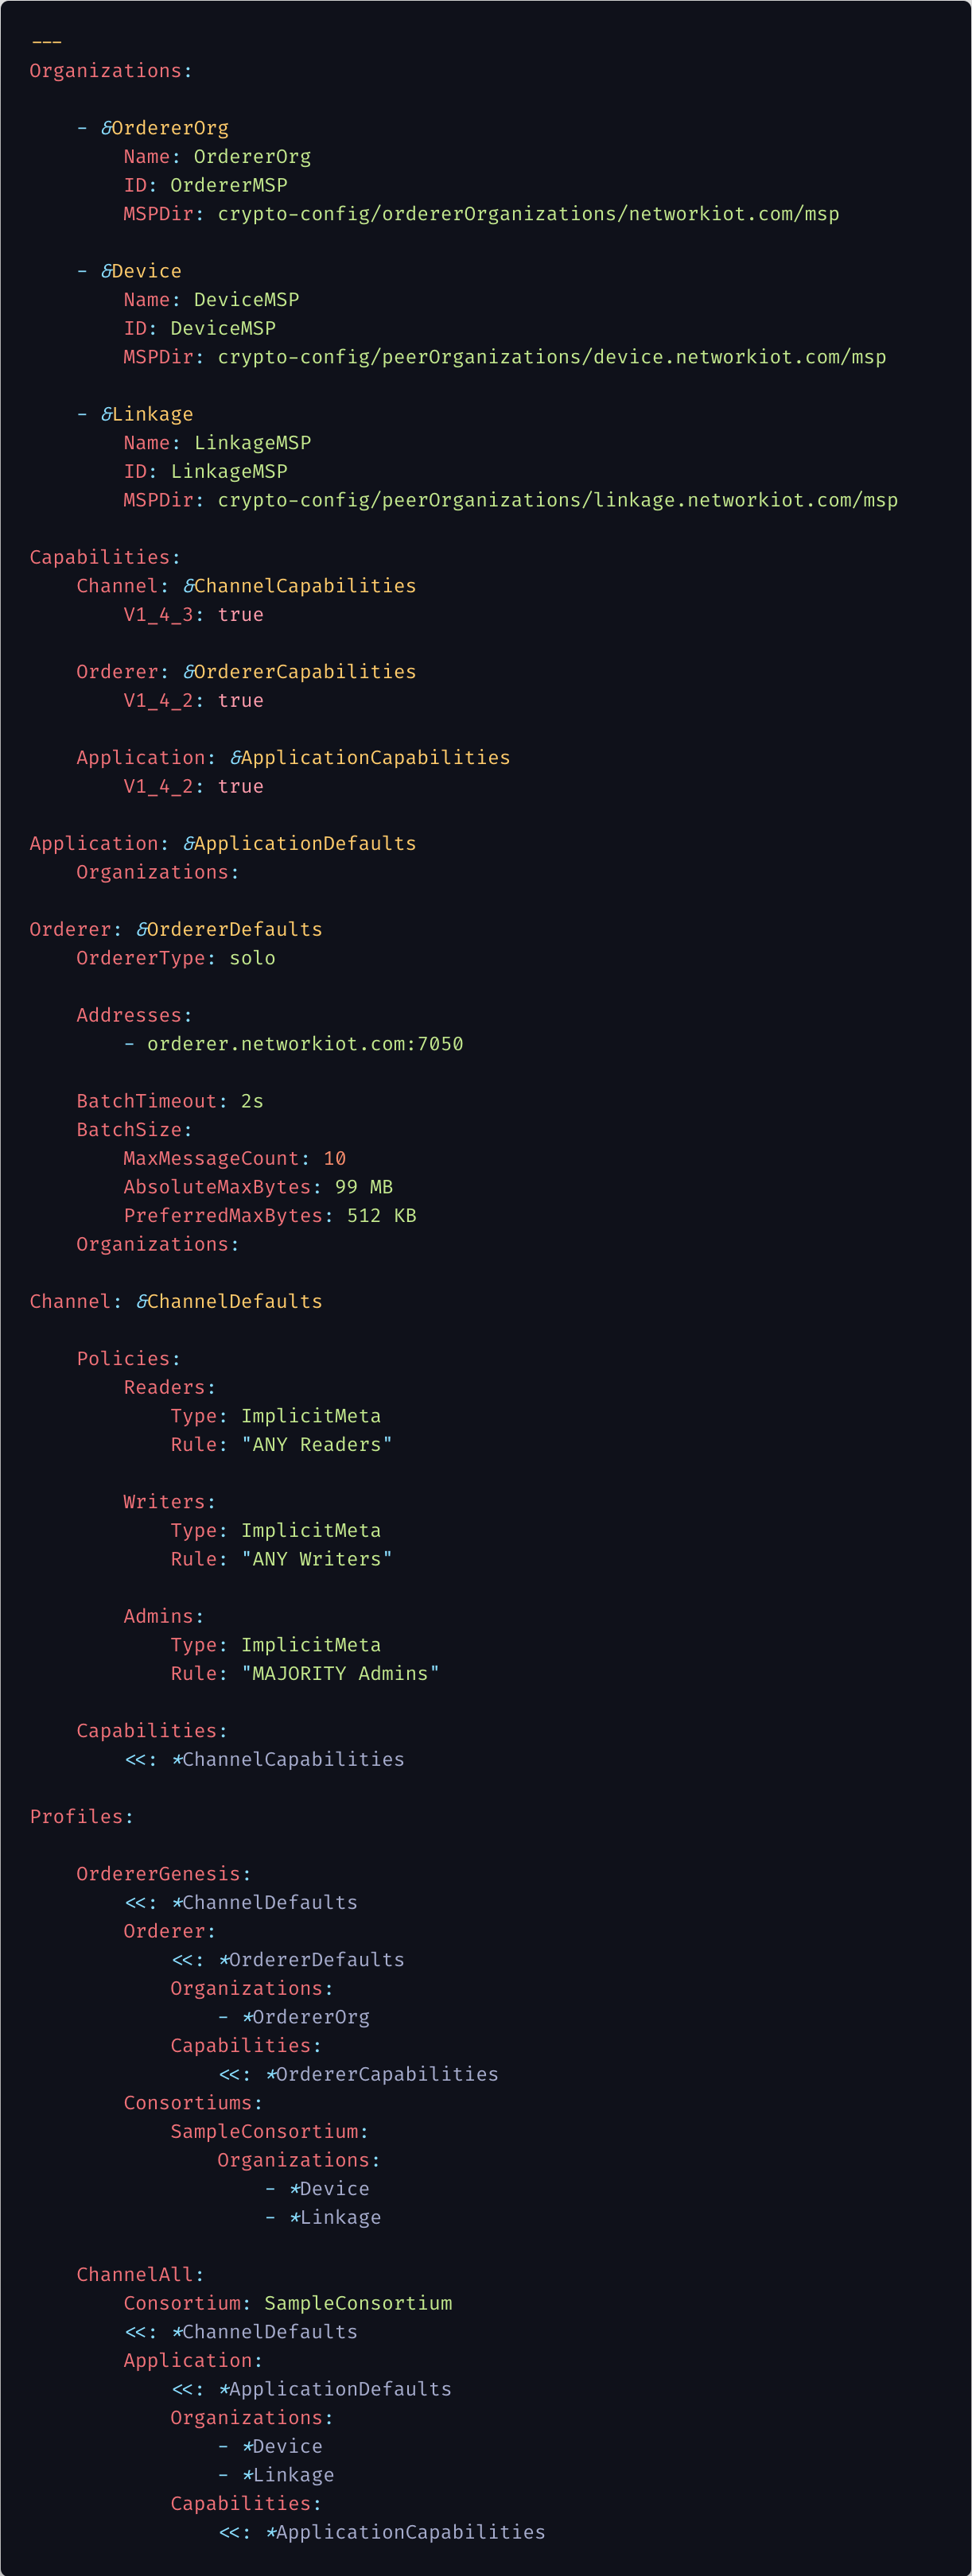
\includegraphics[width=10cm]{imagenes/desarrollo/configtx}
  \caption{Configtx de la red Blockchain.}
  \label{fig:configtx-blockchain}
\end{figure}

\begin{figure}[ht!]
  \centering
  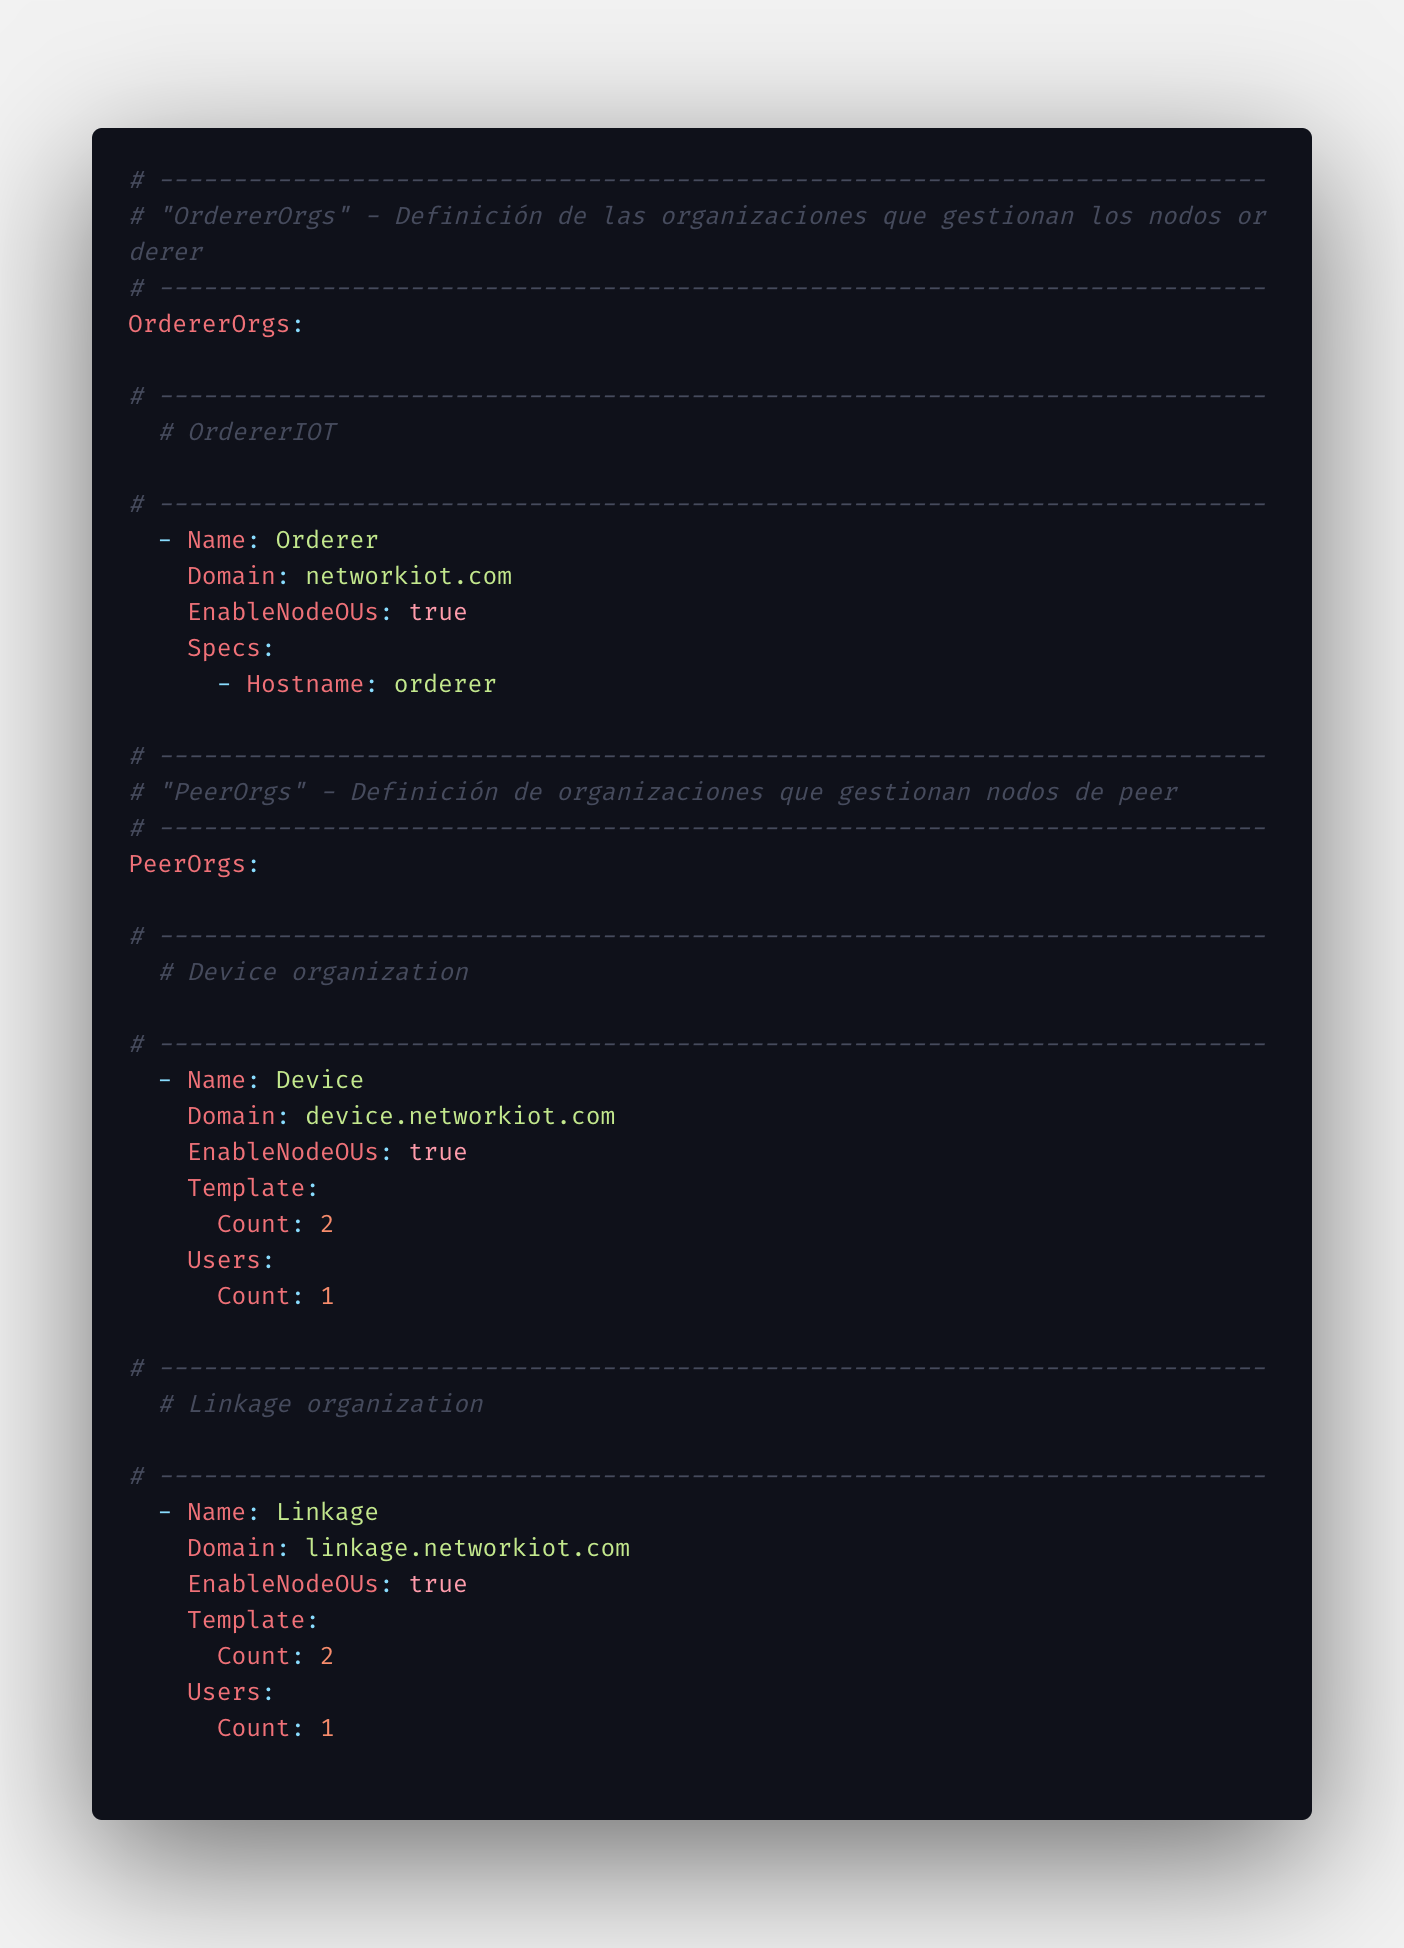
\includegraphics[width=10cm]{imagenes/desarrollo/crypto-config}
  \caption{Crypto-config de la red Blockchain.}
  \label{fig:crypto-config-blockchain}
\end{figure}

\subsubsection{Arquitectura de la red Blockchain.}

\begin{figure}[ht!]
  \centering
  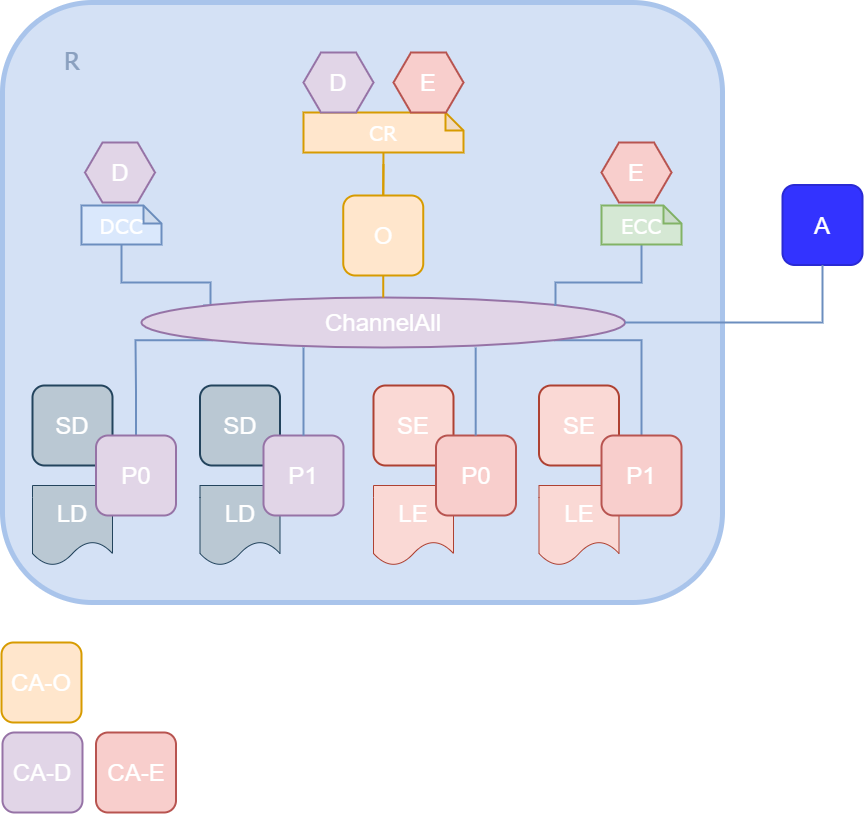
\includegraphics[width=10cm]{imagenes/desarrollo/arquitectura_networkiot}
  \caption{Arquitectura de la red Blockchain.}
  \label{fig:arquitectura-blockchain}
\end{figure}

\begin{figure}[ht!]
  \centering
  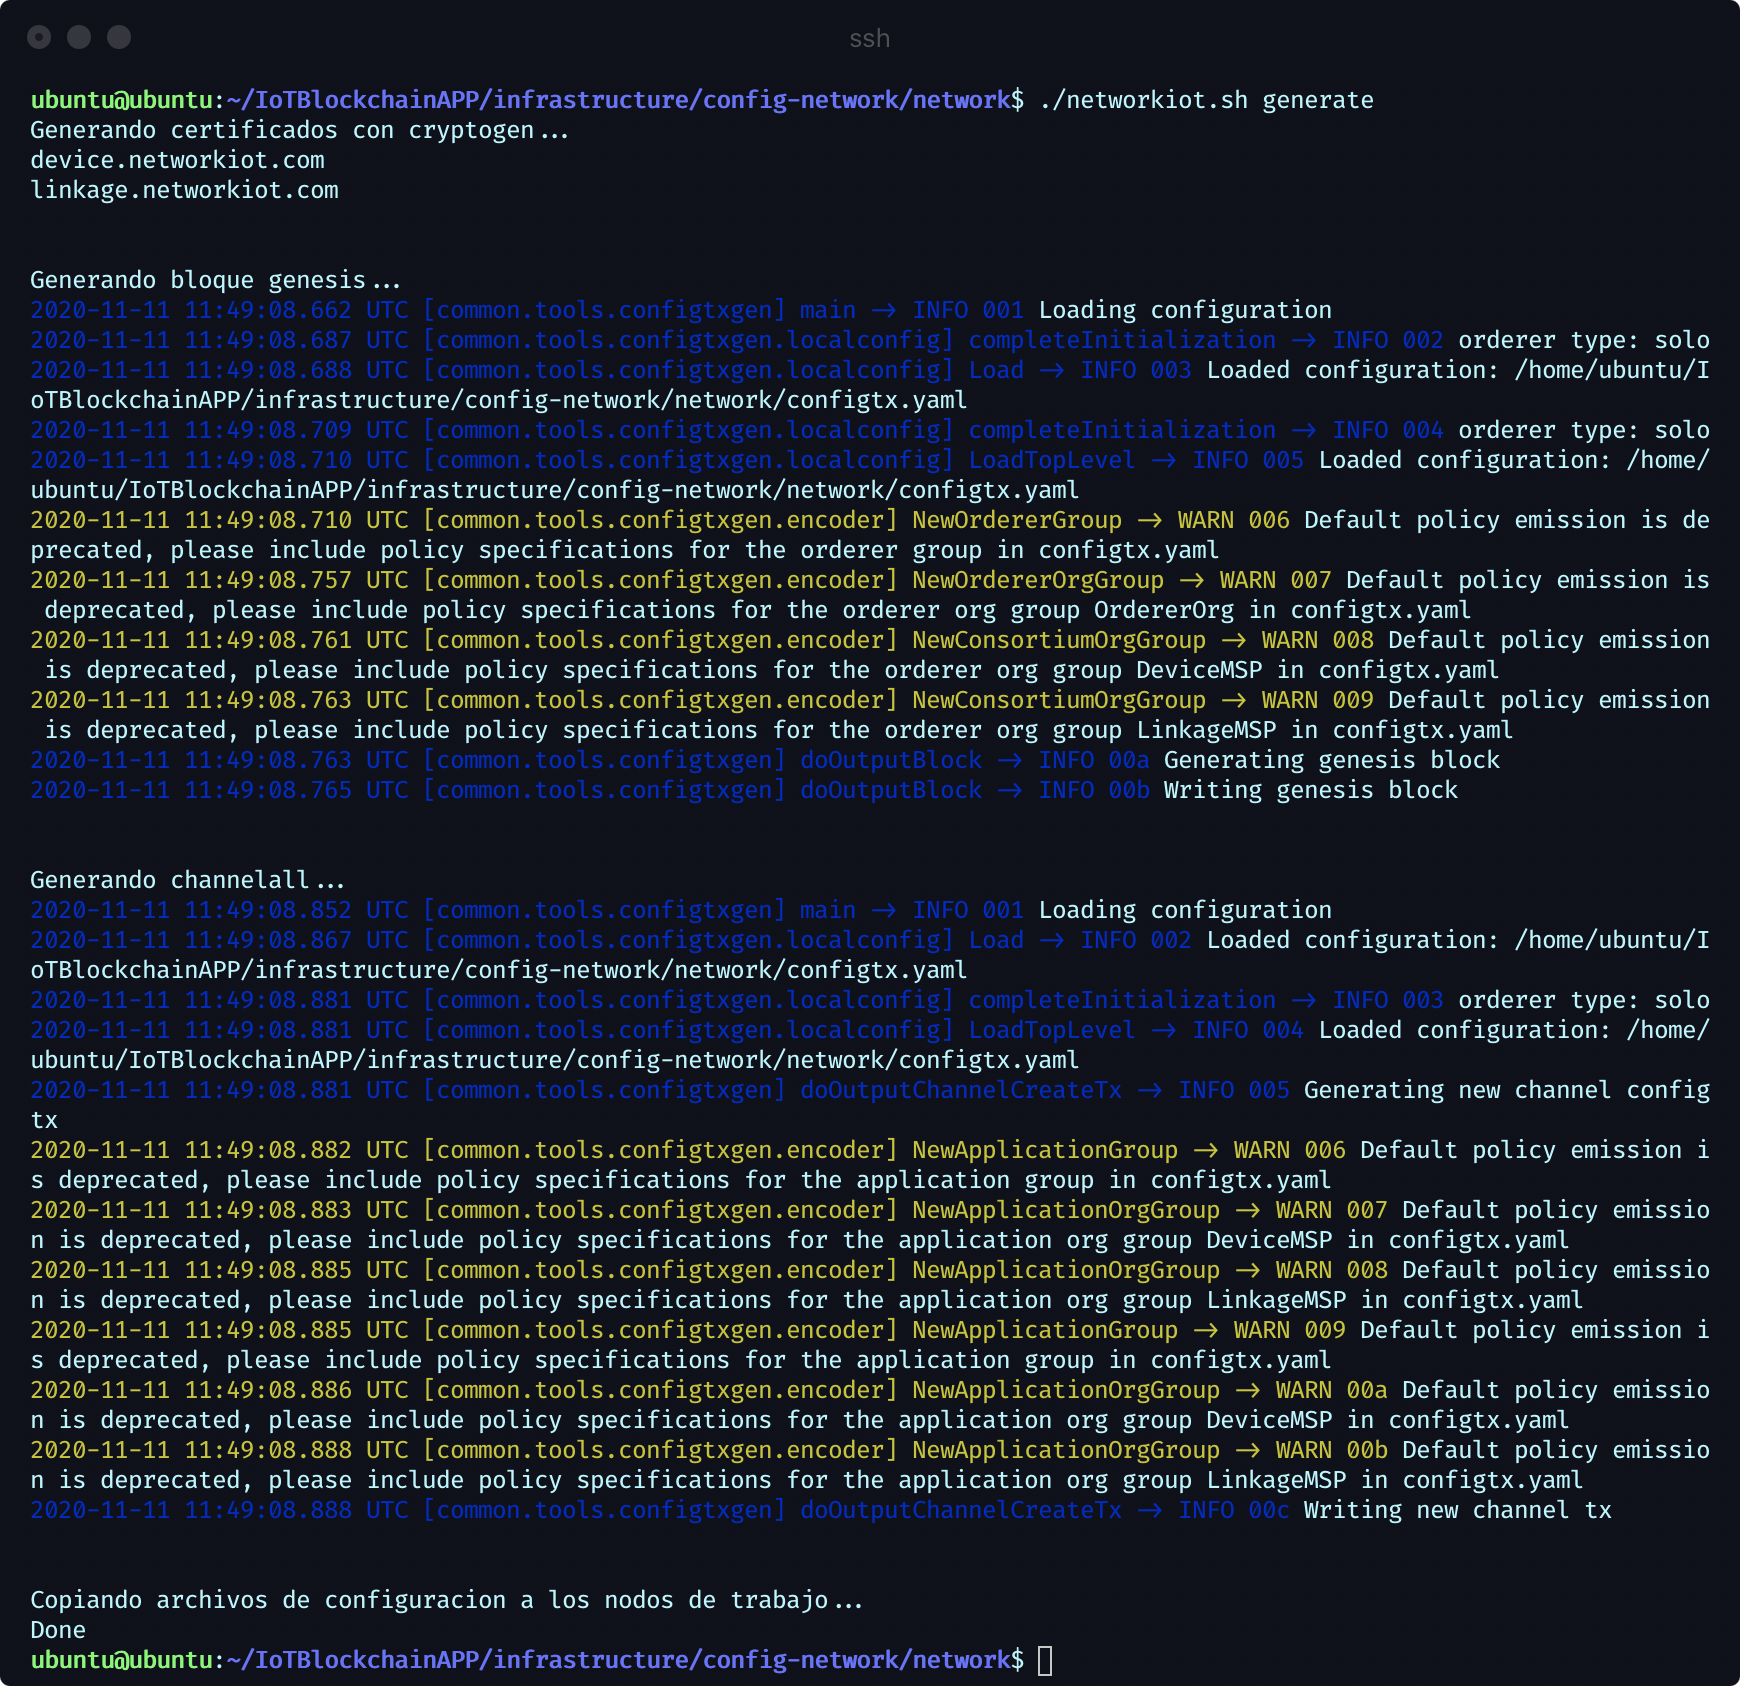
\includegraphics[width=10cm]{imagenes/desarrollo/comandos/generate}
  \caption{Opción generate del script networkiot.}
  \label{fig:generate}
\end{figure}

\begin{figure}[ht!]
  \centering
  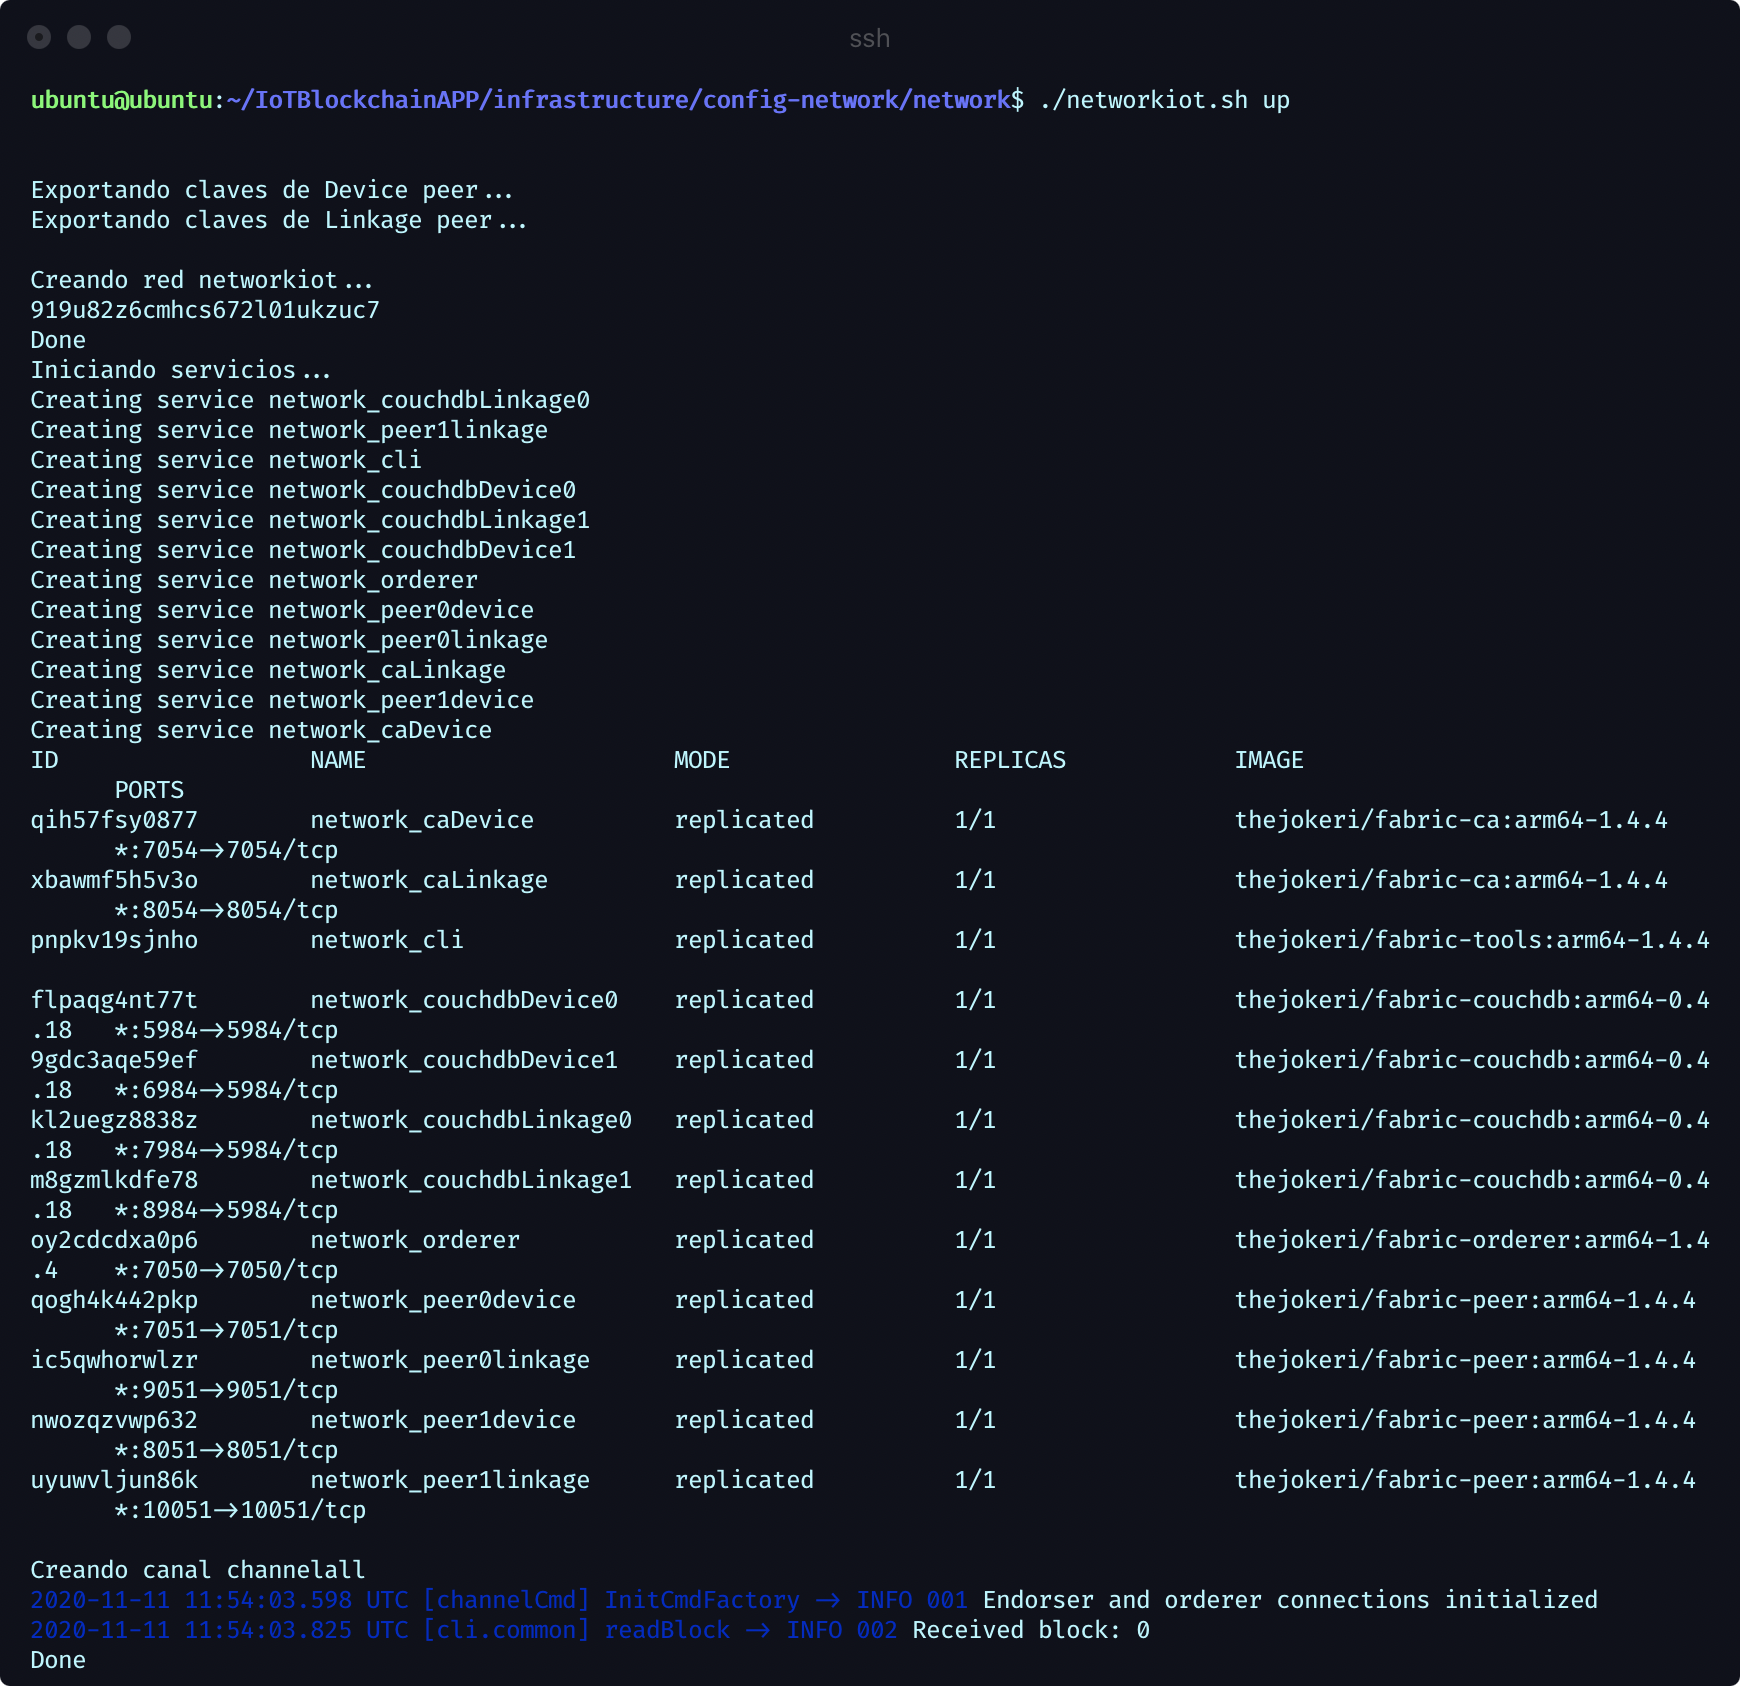
\includegraphics[width=10cm]{imagenes/desarrollo/comandos/up_1}
  \caption{Salida 1 de la opción up del script networkiot.}
  \label{fig:up-1}
\end{figure}

\begin{figure}[ht!]
  \centering
  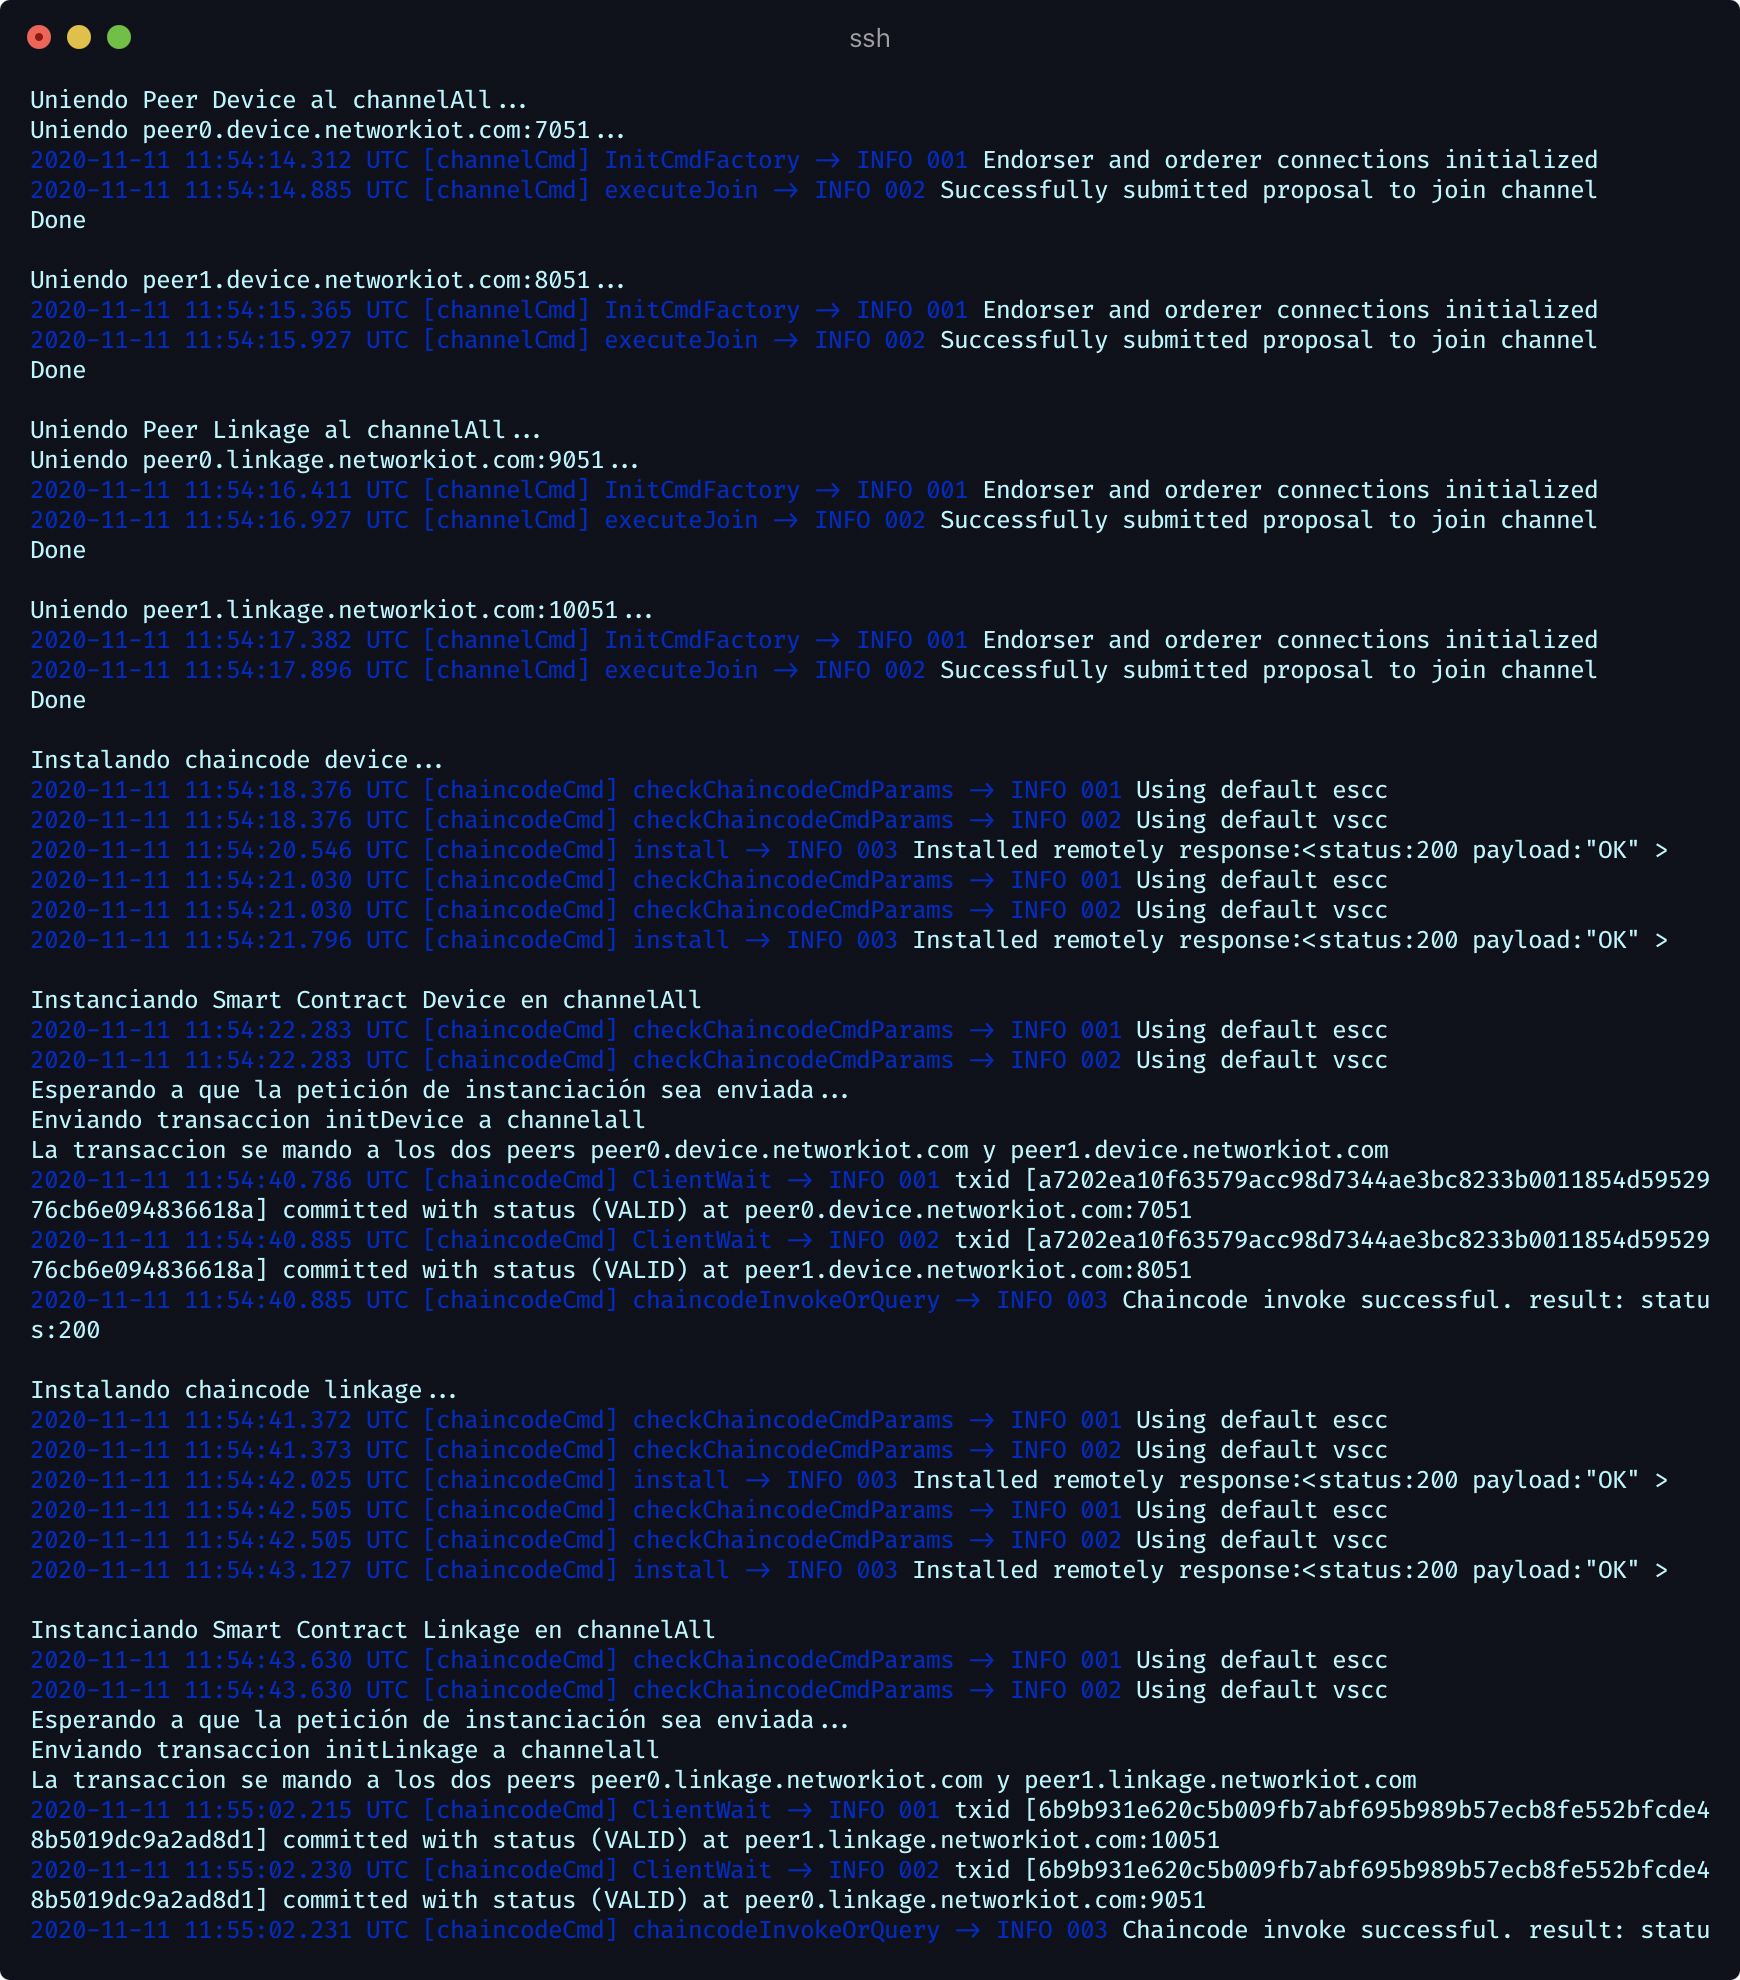
\includegraphics[width=10cm]{imagenes/desarrollo/comandos/up_2}
  \caption{Salida 2 de la opción up del script networkiot.}
  \label{fig:up-2}
\end{figure}

\begin{figure}[ht!]
  \centering
  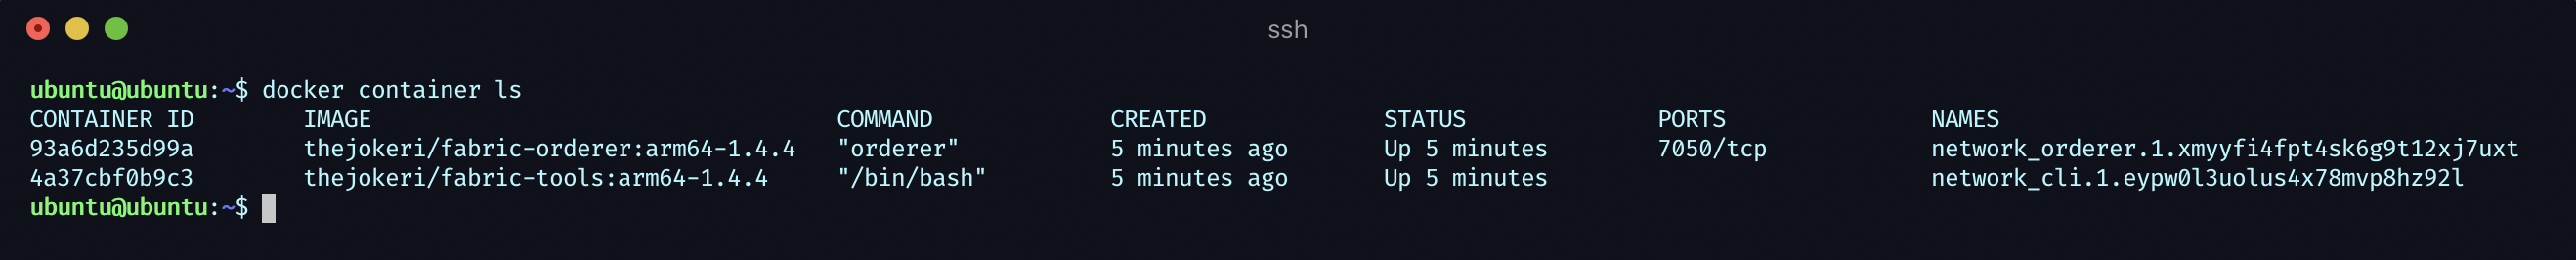
\includegraphics[width=10cm]{imagenes/desarrollo/comandos/containers_master}
  \caption{Salida de contenedores en el nodo maestro.}
  \label{fig:containers-master}
\end{figure}

\begin{figure}[ht!]
  \centering
  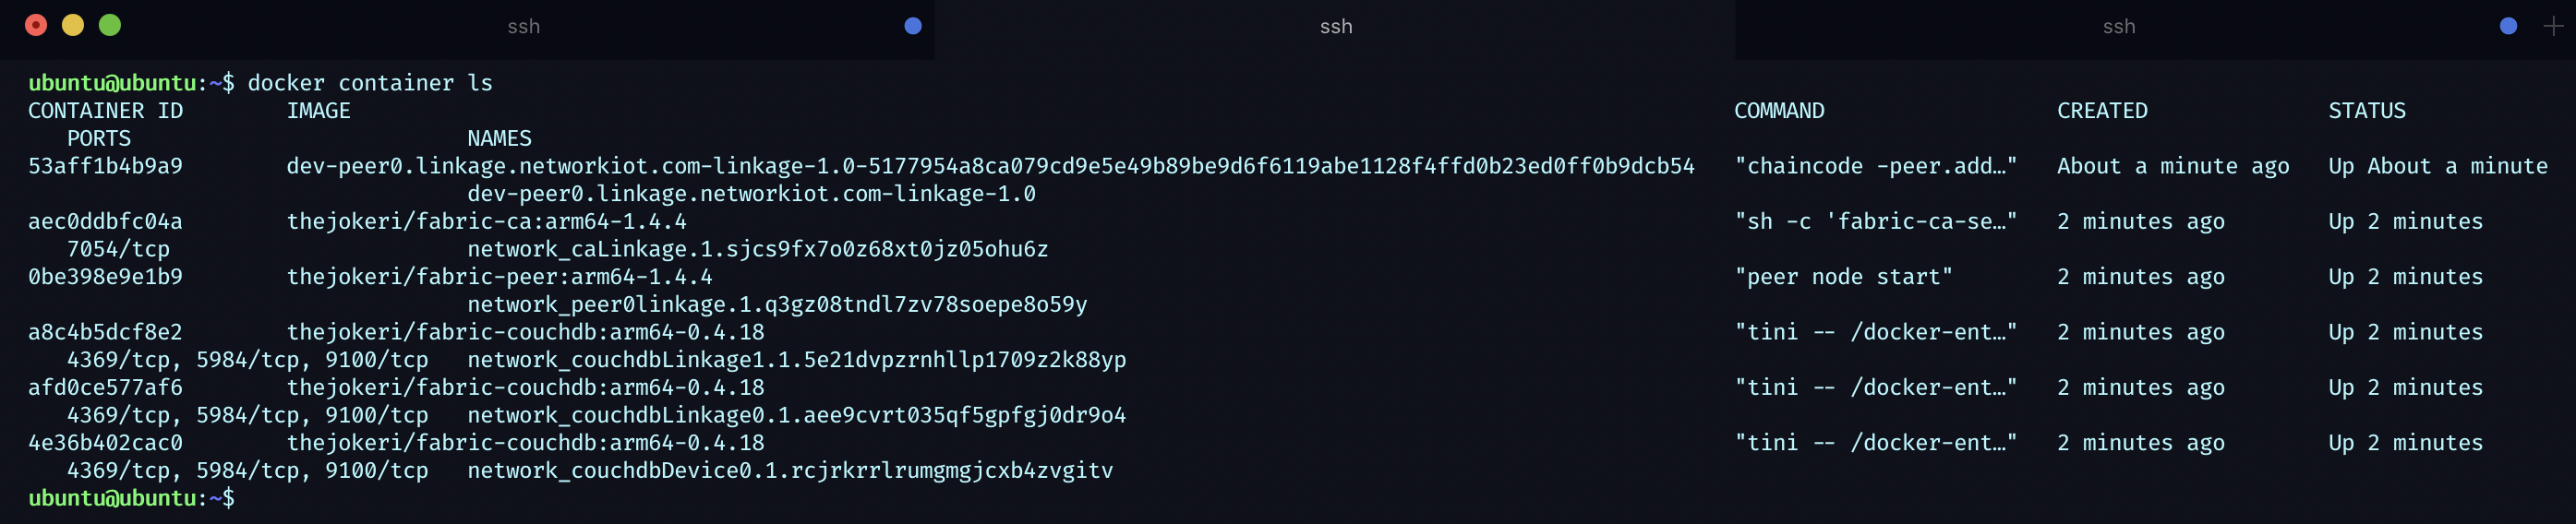
\includegraphics[width=10cm]{imagenes/desarrollo/comandos/containers_worker1}
  \caption{Salida de contenedores en el nodo worker 1.}
  \label{fig:containers-worker1}
\end{figure}

\begin{figure}[ht!]
  \centering
  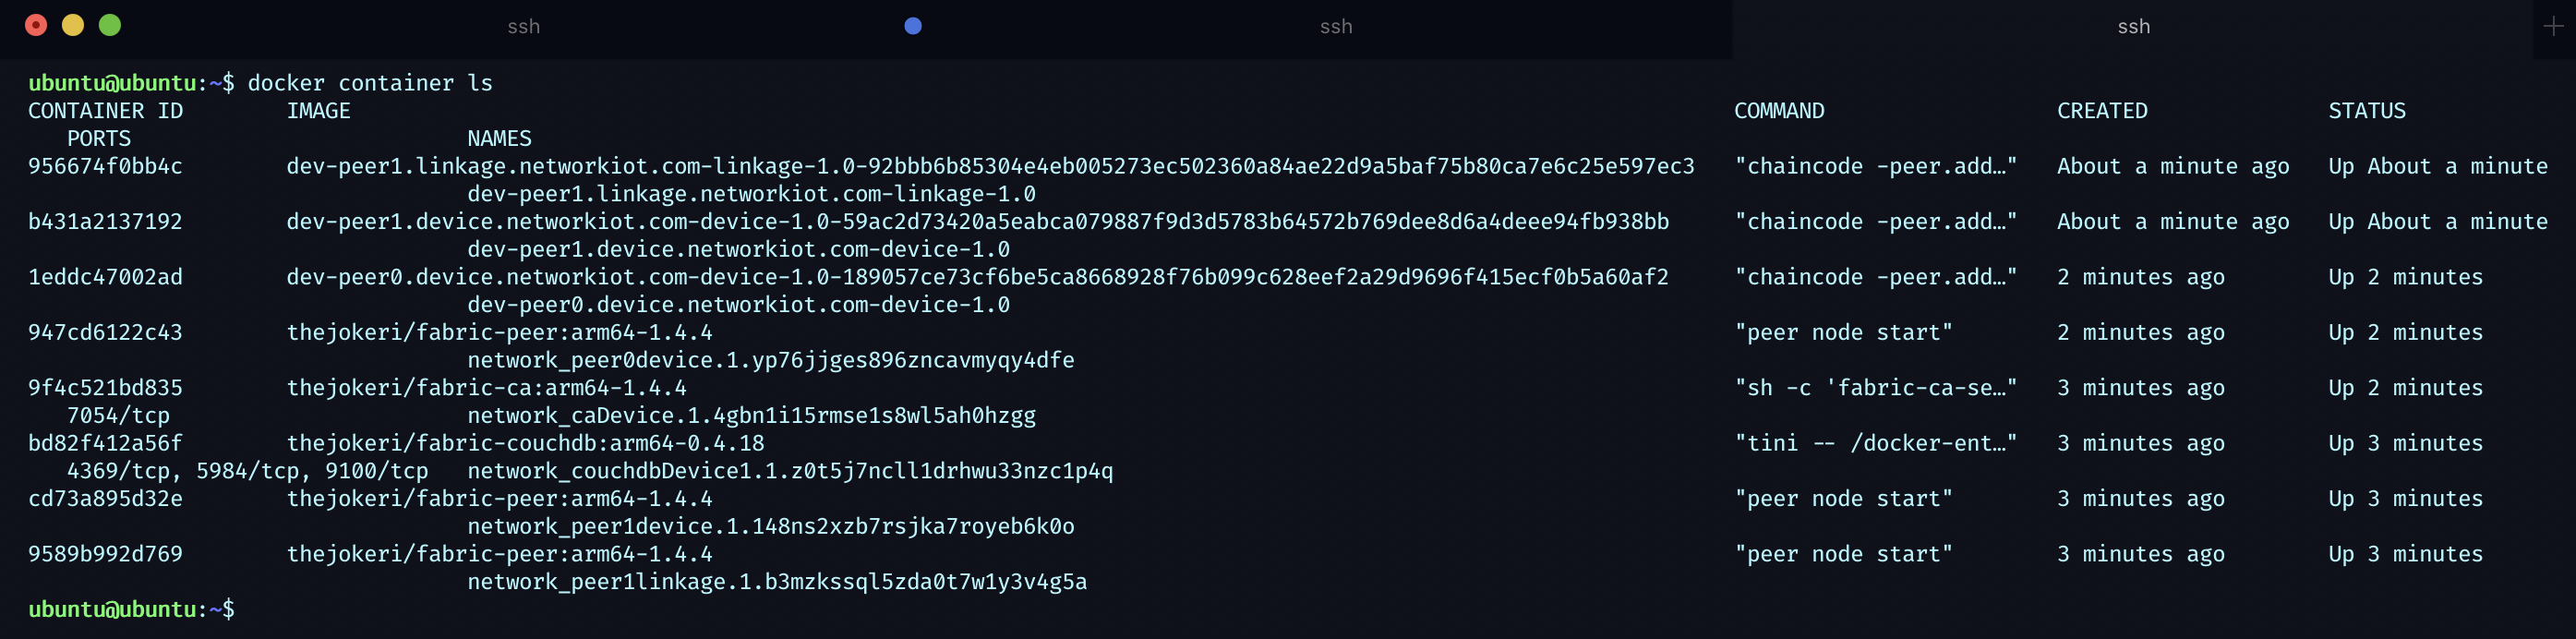
\includegraphics[width=10cm]{imagenes/desarrollo/comandos/containers_worker2}
  \caption{Salida de contenedores en el nodo worker 2.}
  \label{fig:containers-worker2}
\end{figure}

\begin{figure}[ht!]
  \centering
  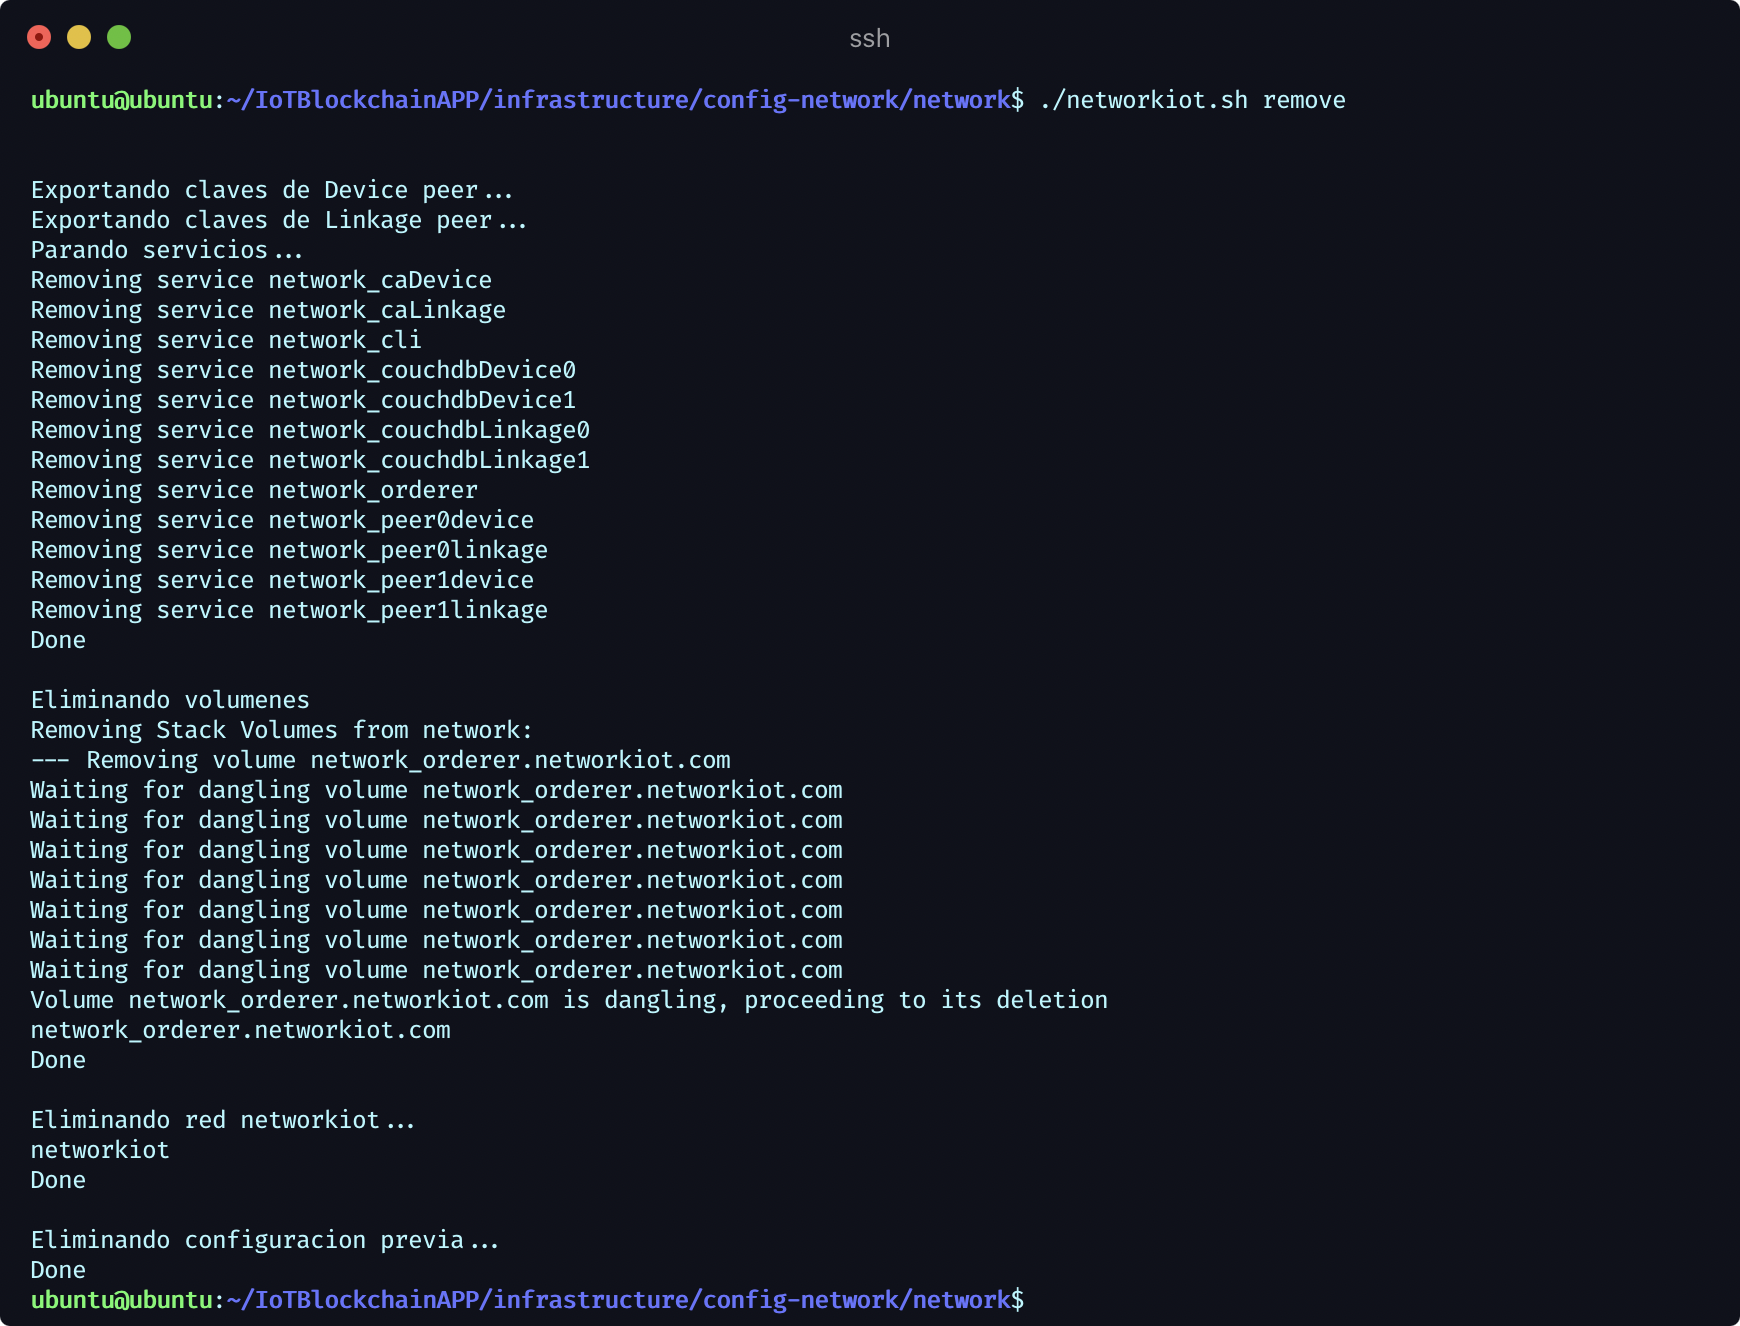
\includegraphics[width=10cm]{imagenes/desarrollo/comandos/remove}
  \caption{Opción remove del script networkiot.}
  \label{fig:remove}
\end{figure}

\subsection{Desarrollo del Back end.}

\begin{figure}[ht!]
  \centering
  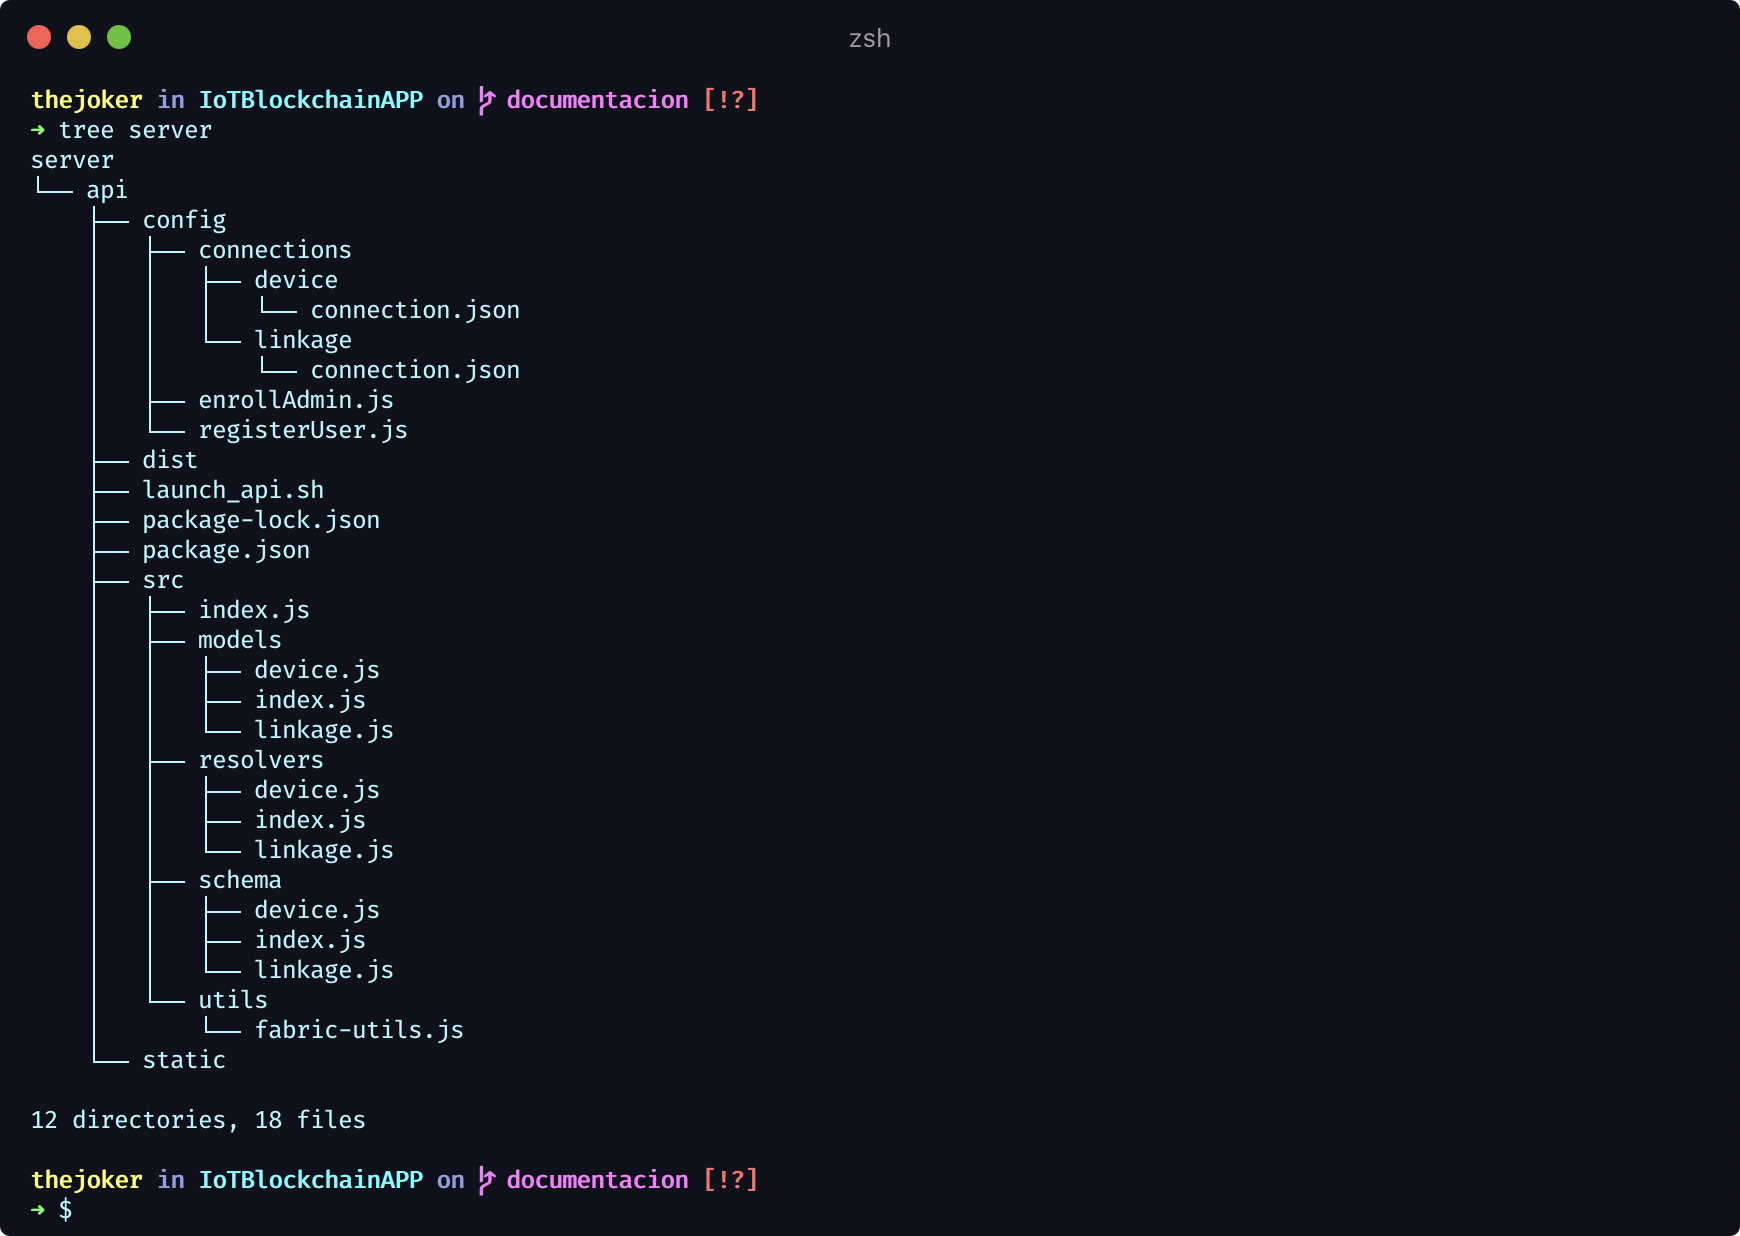
\includegraphics[width=10cm]{imagenes/desarrollo/tree_server}
  \caption{Tree de la carpeta server.}
  \label{fig:tree-server}
\end{figure}

\begin{figure}[ht!]
  \centering
  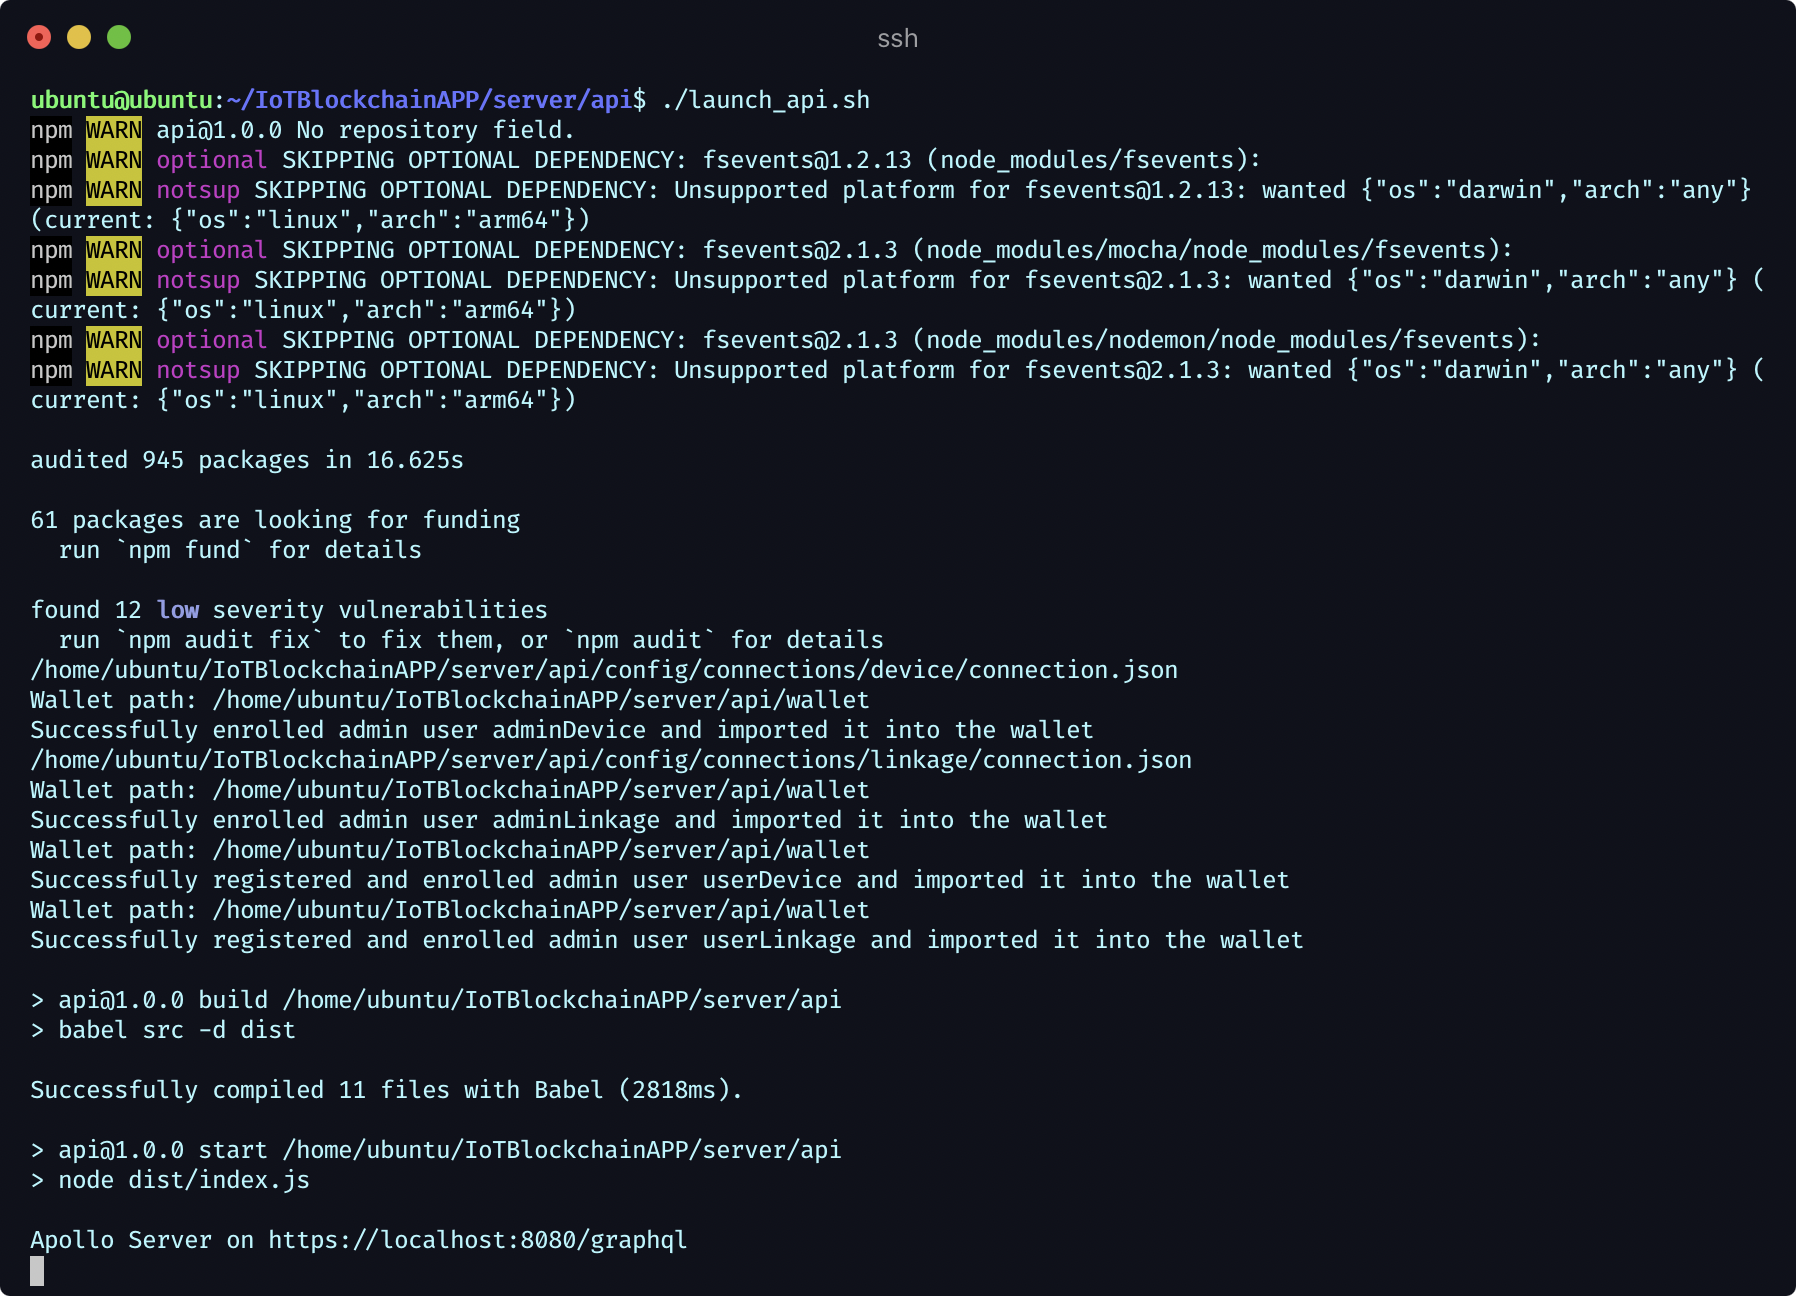
\includegraphics[width=10cm]{imagenes/desarrollo/comandos/launch_api}
  \caption{Ejecución del script launch\_api.}
  \label{fig:launch-api}
\end{figure}

\subsection{Desarrollo del Front end y despliegue.}

\begin{figure}[ht!]
  \centering
  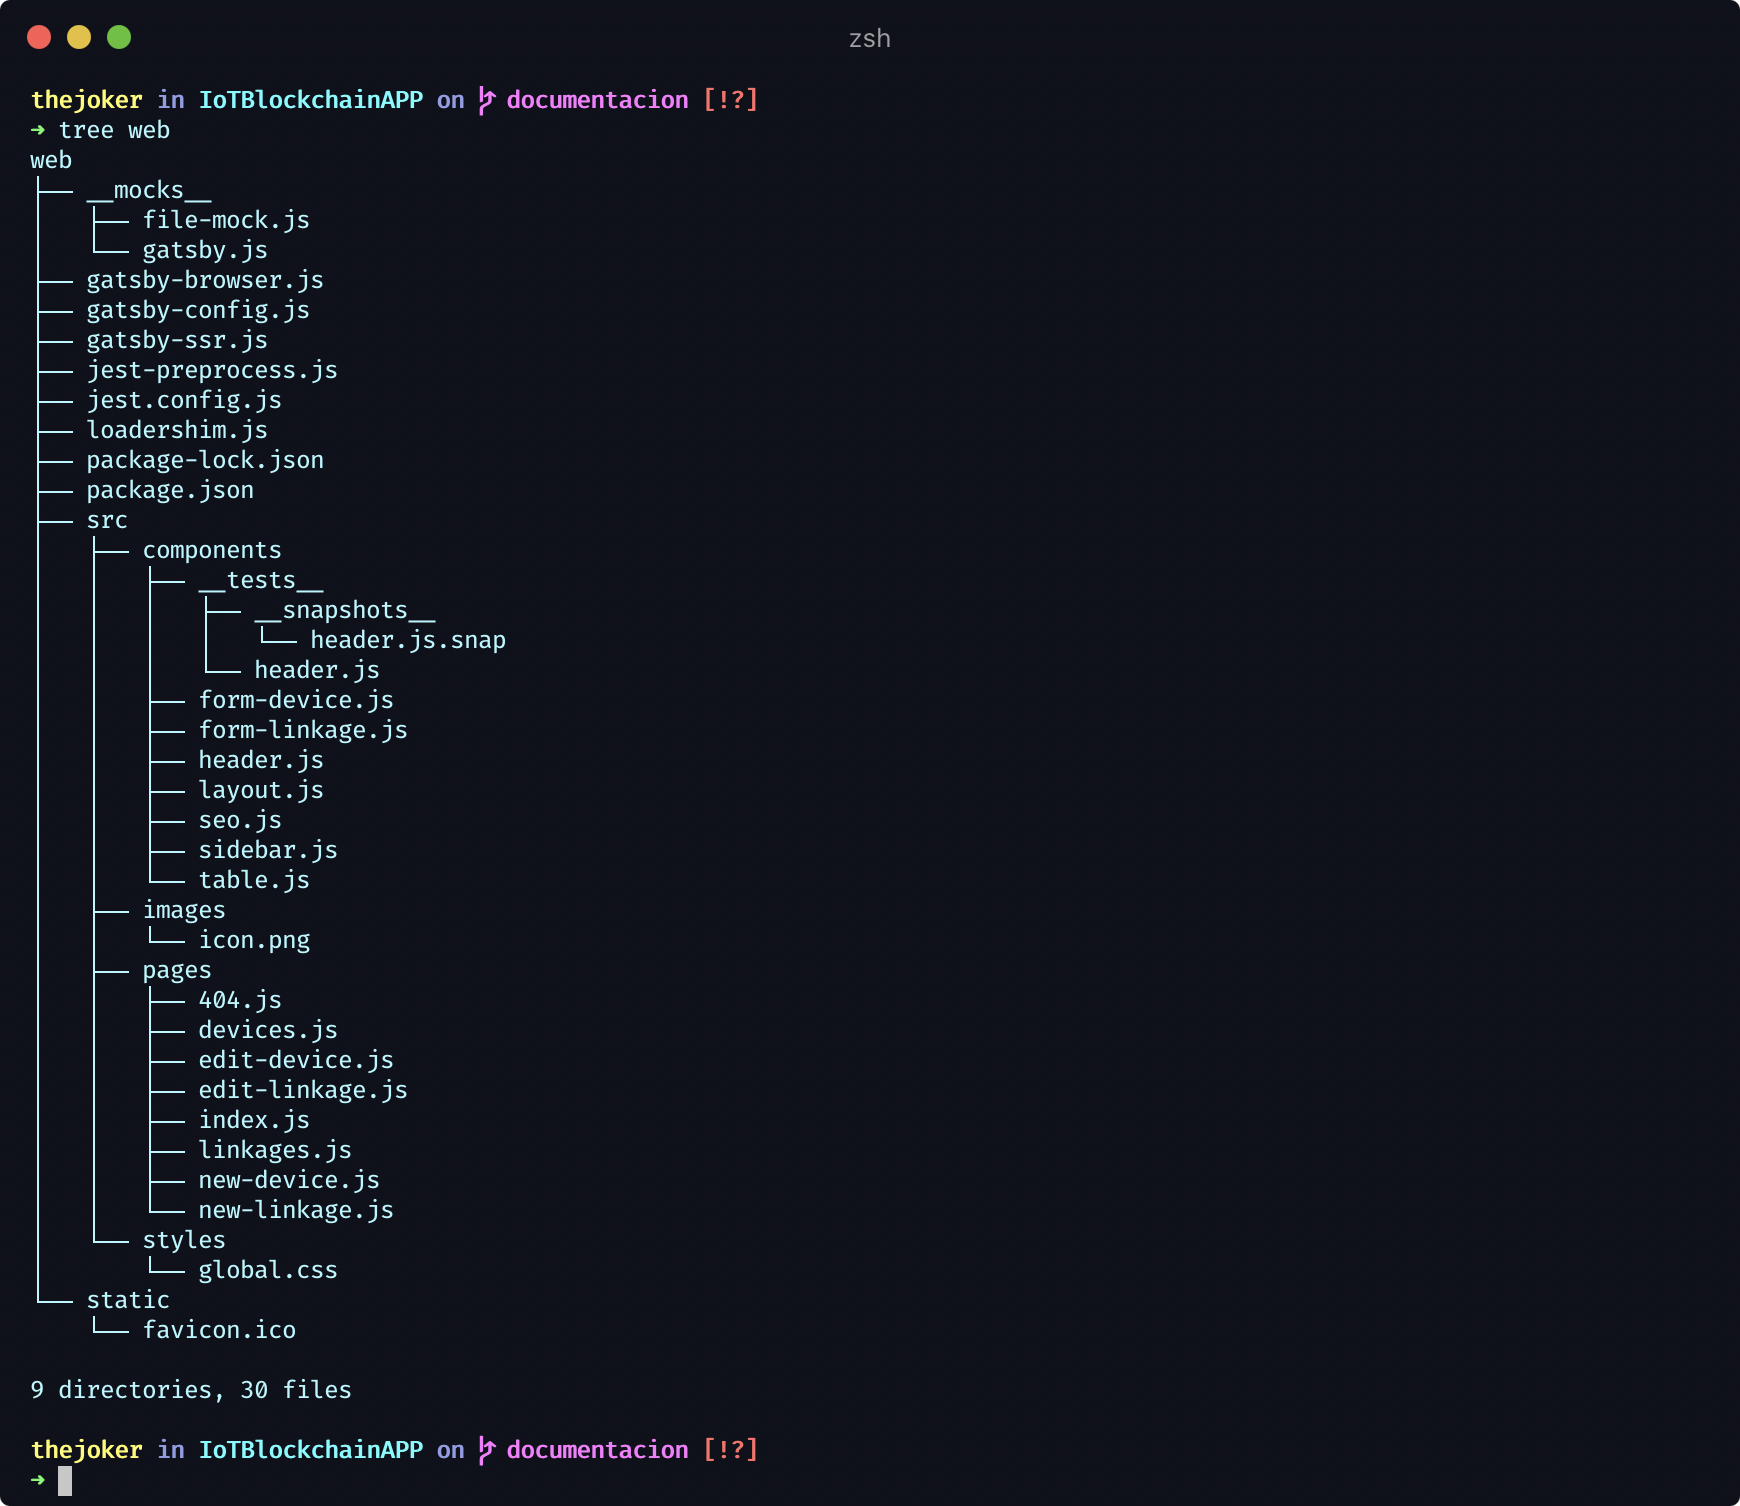
\includegraphics[width=10cm]{imagenes/desarrollo/tree_web}
  \caption{Tree de la carpeta web.}
  \label{fig:tree-web}
\end{figure}

\subsection{Conclusión.}

\newpage
\section{Conclusiones.}

\newpage

\section{Trabajos futuros.}

\newpage

\myemptypage

\section{Bibliografia y webgrafía}
\printbibliography

\end{document}
